\clearpage
\section{Apps \& Navigation}
\label{sec:builder-feature-navigation}

The “Apps \& Navigation” page decides what members see in the app list and in what order. It shows navigation as a three-level tree: the app, then its sections, then the modules inside each section. A module is any item a member opens from the menu: a record type, a form, a dashboard, a page or a page built into the system.

From this page you reorder items by dragging and show or hide them with their switches. These edits do not reach members at once; they stay as a draft on the page until you press “Save changes”, so you can try an order and undo it safely.

\textbf{Path and who uses it:} “Builder” → “Core” → “Apps \& Navigation”. Available only to the organization owner and administrator.

\begin{rcnote}[Example: Horizon]
The system administrator adds a “Branch services” app with a “Visits” section, drags “Visit requests” into it and saves, so Omar Haddad finds it in the app list on his next page load. They add the app from ① and save from ⑤.
\end{rcnote}

\begin{figure}[H]
\centering
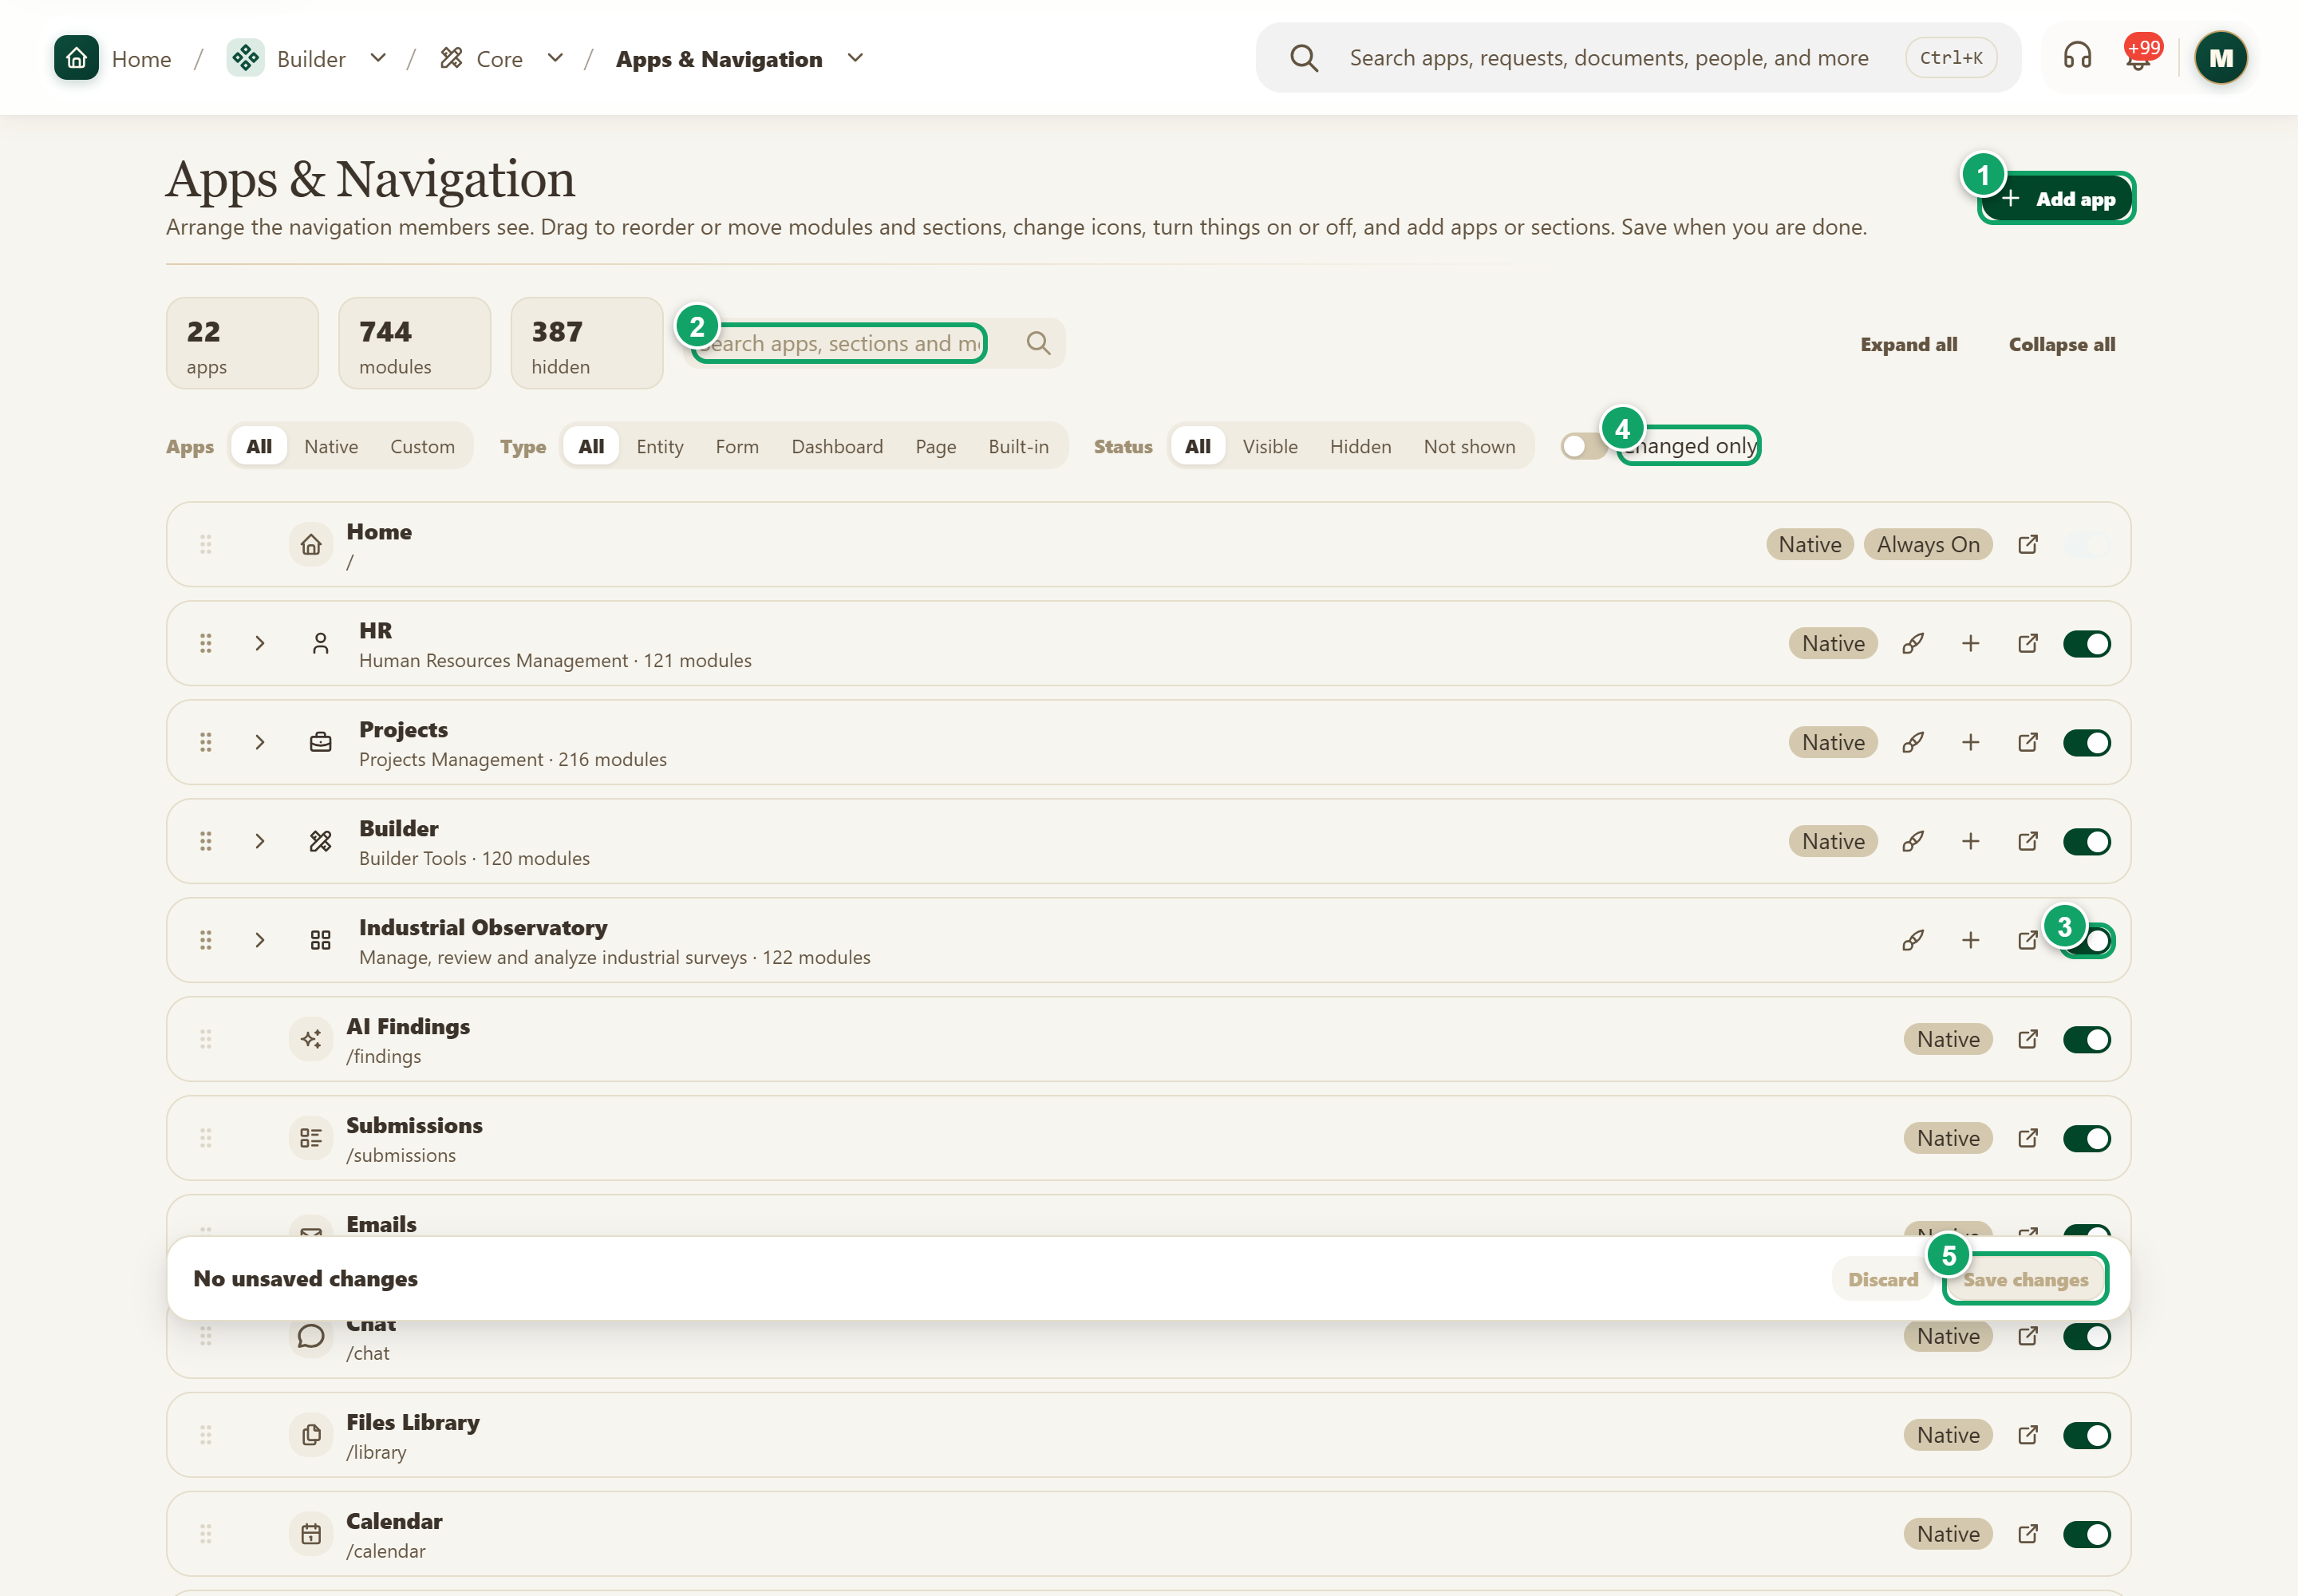
\includegraphics[width=0.95\linewidth,height=0.72\textheight,keepaspectratio]{figures/screens/ch06-navigation-en.png}
\caption{The “Apps \& Navigation” page}
\label{fig:builder-navigation-screen}
\shotnote{The image shows the “Apps & Navigation” page in the test organization, with 22 apps, each with its chips and visibility switch. Order and switch changes stay a draft whose state the save bar shows until you save, so you can review them before they reach members. ① “Add app”: creates a new app and saves it at once. ② Search: finds an app, section or module by name. ③ The app switch: shows or hides it with everything in it. ④ “Changed only”: shows what you changed and have not saved. ⑤ “Save changes”: saves order and switches.}
\end{figure}

\begin{table}[H]
\centering
\caption{Parts of the page}
\label{tab:builder-navigation-data}
\begin{tabularx}{\linewidth}{R{3.6cm} Y}
\rcHeaderRow
\thh{Part} & \thh{Content and action}\\
Counts and search & The page shows the number of “apps”, “modules” and “hidden” items. The search “Search apps, sections and modules” finds any item by name, and “Expand all” and “Collapse all” open or fold the apps.\\
Filters & “Apps”: “All”, “Native” or “Custom”; “Type”: “Entity”, “Form”, “Dashboard”, “Page” or “Built-in”; “Status”: “Visible”, “Hidden” or “Not shown”; then “Changed only” to show what you changed and have not saved. “Clear filters” brings back the full list.\\
Dragging & Drag an app by its handle to change its order, drag a section within its app or to another app, and drag a module within its section or to another section.\\
Switches & A switch shows or hides the item. Hiding an app or section hides everything in it.\\
Save bar & Shows the number of unsaved changes, with “Discard” to undo them and “Save changes” to save them.\\
How changes take effect & Reminds you that modules keep their visibility on their own records: record types, forms and dashboards in “Show in navigation”, and pages in their published status.\\
\end{tabularx}
\end{table}

\begin{table}[H]
\centering
\caption{Chips on the tree rows}
\label{tab:builder-navigation-chips}
\begin{tabularx}{\linewidth}{R{3.6cm} Y}
\rcHeaderRow
\thh{Chip} & \thh{What it means}\\
Native & An app built into the system, such as Email and Chat. These apps can only be turned on or off and do not receive new modules.\\
Always on & An app that cannot be turned off, such as Settings and Home, so its switch is disabled.\\
Hidden or Draft & The module itself is off. “Draft” shows for a page that is not published yet.\\
Off · inherited & The module is on, but its app or section is off, so members do not see it until you turn the parent on.\\
\end{tabularx}
\end{table}

\begin{rcwarn}[Where can a module move?]
A module can only move to a section that has a record: a section added on this page or saved as a record. If you drop a module on a built-in section, the message “That app or section is built in and cannot receive modules. Move it to a section that has a record.” appears and nothing changes. Built-in modules without a record cannot be dragged at all; you can only hide them.
\end{rcwarn}

\begin{figure}[H]
\centering
\begin{tikzpicture}[node distance=0.5cm]
\node[entity] (app) {App};
\node[entity,below=0.7cm of app] (section) {Section};
\node[entityOpt,below right=0.7cm and 0.3cm of section] (type) {Record type or form};
\node[entityOpt,below left=0.7cm and 0.3cm of section] (dash) {Dashboard or page};
\draw[dependsOn] (app) -- (section);
\draw[dependsOnOpt] (section.south) -- ++(0,-0.3) -| (type.north);
\draw[dependsOnOpt] (section.south) -- ++(0,-0.3) -| (dash.north);
\end{tikzpicture}
\rclegend
\caption{How navigation is built}
\label{fig:builder-navigation-tree}
\shotnote{The figure shows that an app holds sections, and a section holds the modules members open, such as record types, forms and dashboards. So create the app and section first and then drag the module into it; a built-in app does not receive new modules.}
\end{figure}

\subsection{Steps and check}
\begin{enumerate}
\item Open “Apps \& Navigation” and type the module's name in the search, or pick its kind in the “Type” filter.
\item Drag the module by its handle to the section you want, and drop it where you want it among the section's modules.
\item Make sure the module's switch and the switches of its section and app are on, and that the row has no “Hidden” or “Off · inherited” chip.
\item Turn on “Changed only” to review what you changed, then press “Save changes”.
\end{enumerate}

\textbf{Check and recovery:} the message “Navigation saved.” should appear, the bar should return to “No unsaved changes”, and members see the new order on their next page load. If an item does not show for a member, check that they can see its records, because a section with no item they are allowed to open is not shown. If “Could not save the changes. Please try again.” appears, check your connection and press “Save changes” again; your edits stay on the page unless you press “Discard”.

\clearpage
\section{Adding apps and sections}
\label{sec:builder-feature-navigation-apps-sections}

When you build new work, no existing app may suit it. The page therefore lets you create a new app to hold this work, then add sections inside it to group its modules. Unlike ordering and switching, this action is saved as soon as you create the item, so you do not need “Save changes” afterwards.

Each app or section only needs a title, a short description and an icon. Later you can change the icon from its row, and delete a section you added if it stays empty.

\textbf{Path and who uses it:} “Builder” → “Core” → “Apps \& Navigation” → “Add app”, or the “Add section” button on an app's row. Used by the organization owner and administrator when launching new work.

\begin{rcnote}[Example: Horizon]
The system administrator presses “Add app”, types the title “Branch services” with a description saying it gathers the services of the Damascus and Aleppo branches, and presses “Create”. Then they add a “Visits” section to the app to hold “Visit requests”. These steps match numbers ① to ④ in the image.
\end{rcnote}

\begin{figure}[H]
\centering
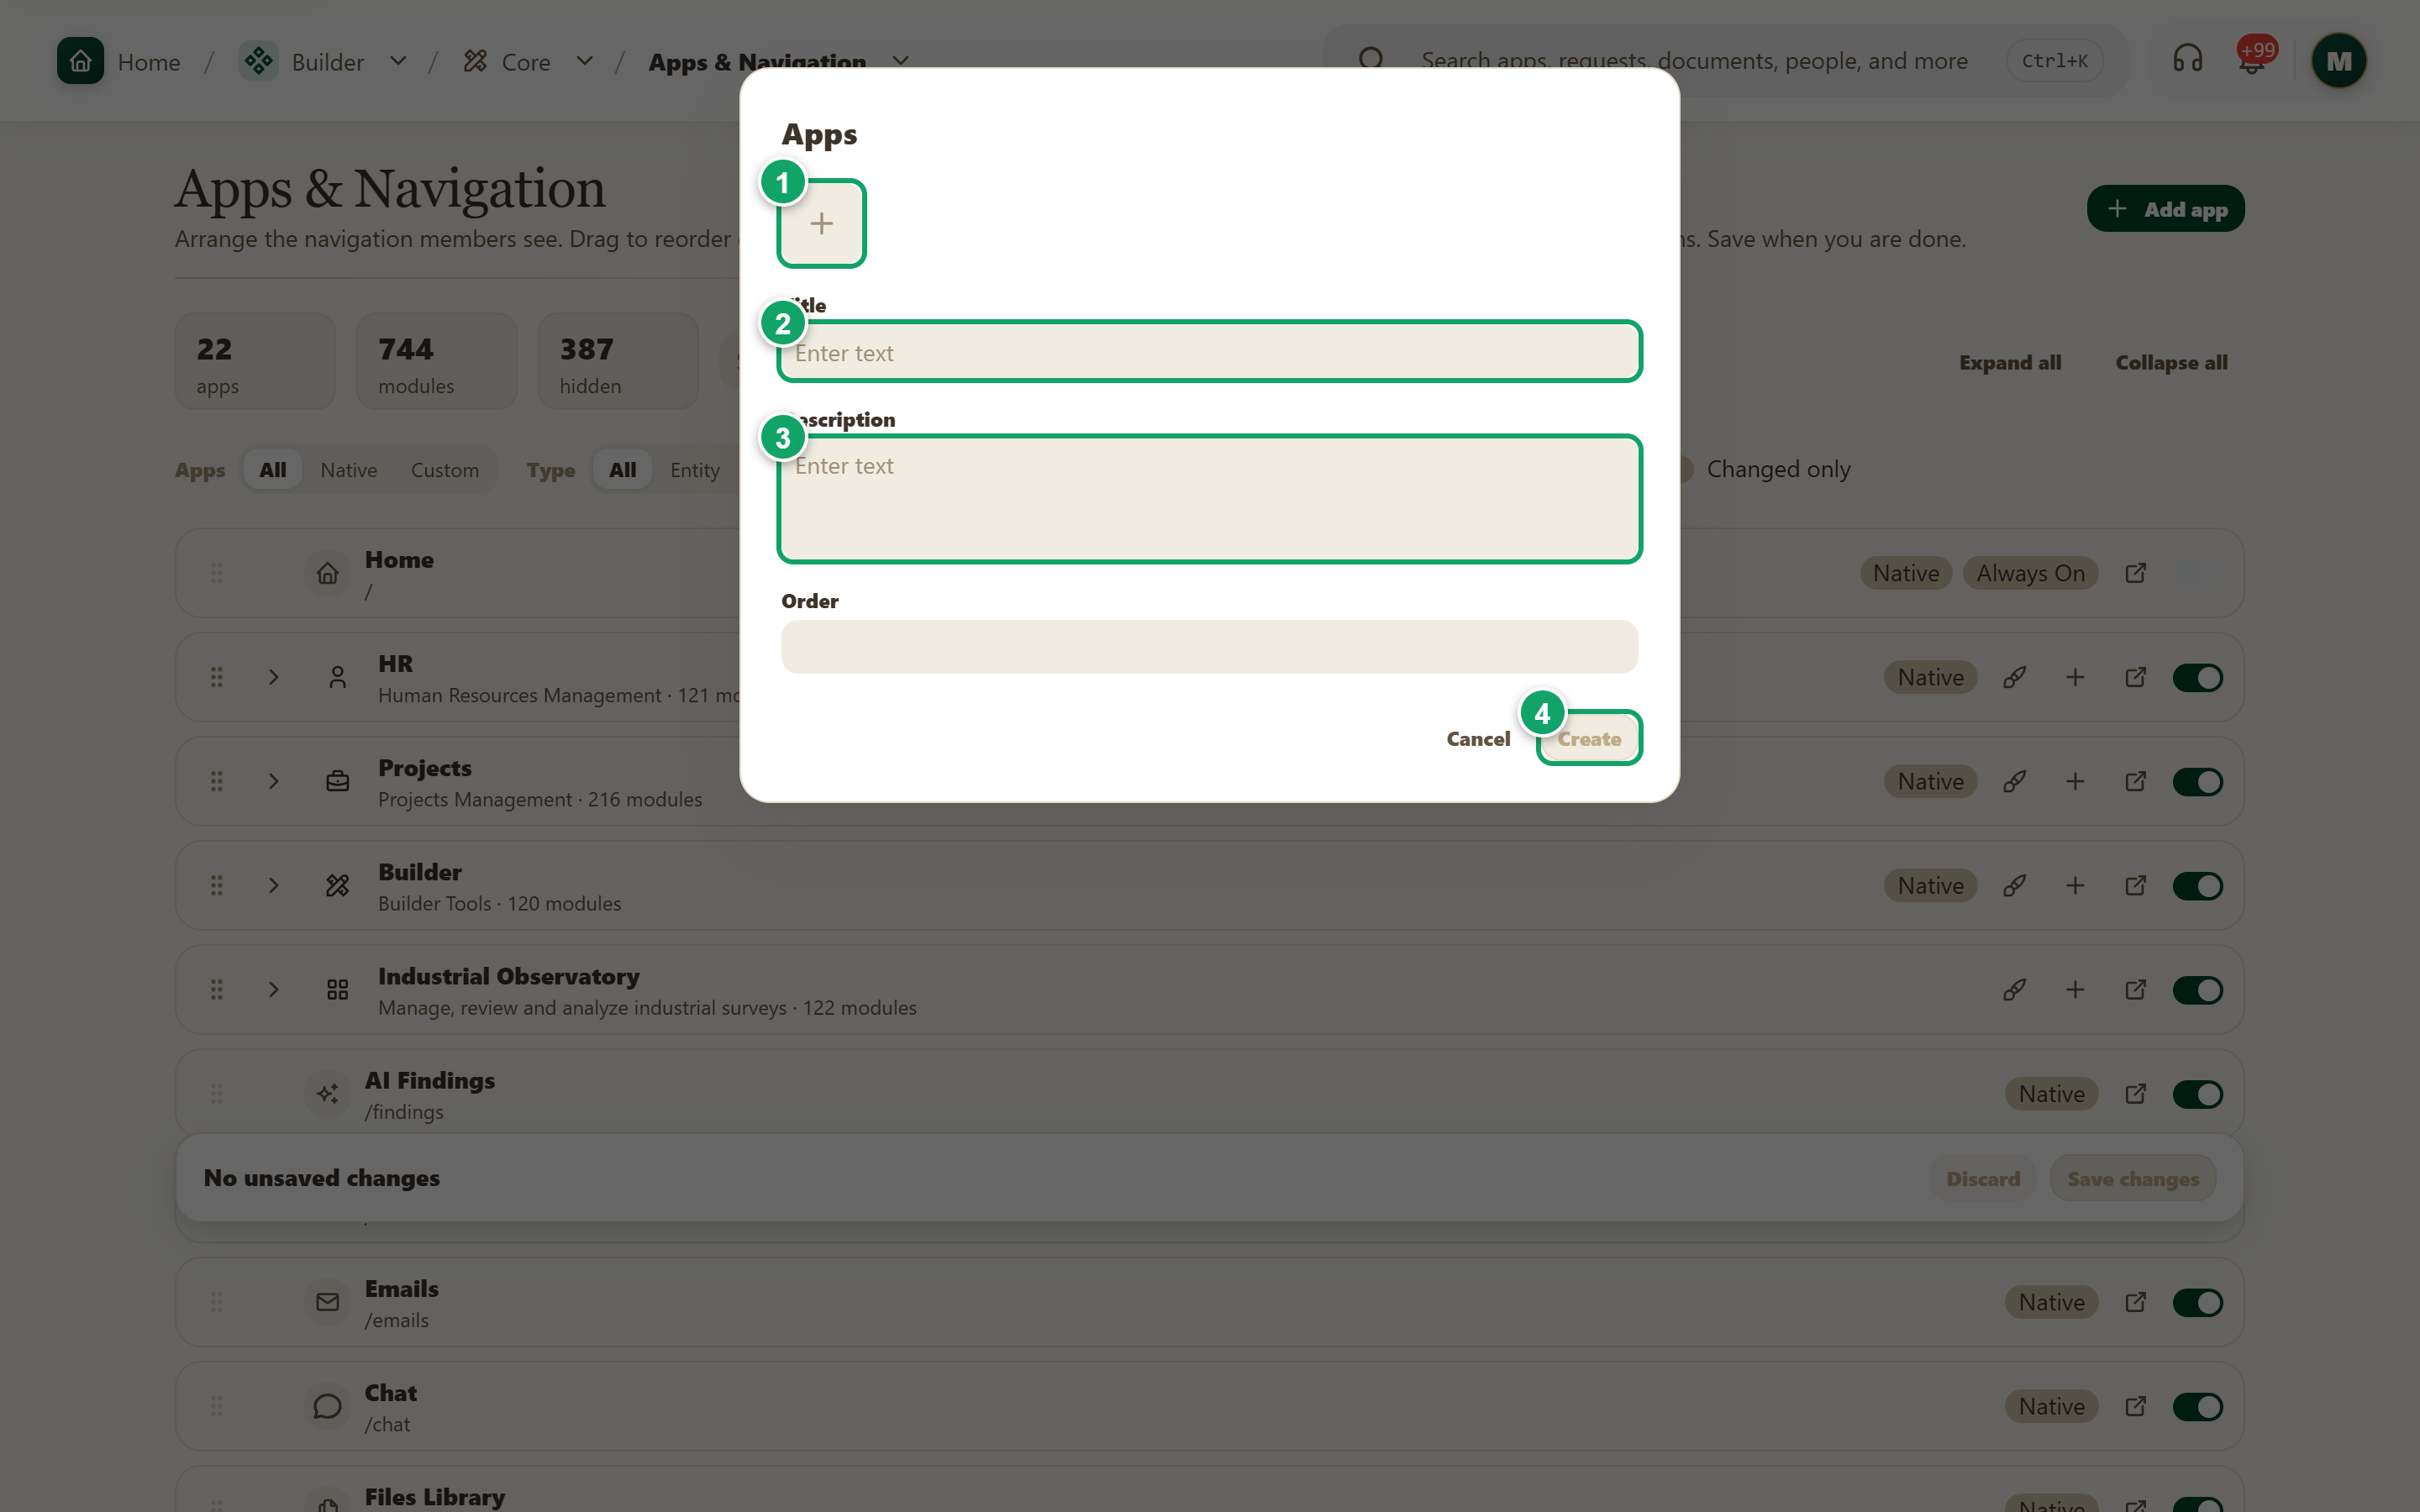
\includegraphics[width=0.95\linewidth,height=0.72\textheight,keepaspectratio]{figures/screens/ch06-nav-add-app-en.png}
\caption{The create dialog before it is filled in}
\label{fig:builder-navigation-apps-sections-screen}
\shotnote{The image shows the dialog that opens after pressing “Add app” in the test organization; it is empty because the capture created nothing. The same dialog opens from the “Add section” button in an app’s row, and what you create is saved as soon as you press “Create”, without “Save changes”. ① The icon picker: chooses the app’s or section’s icon. ② “Title”: the name shown in the menu. ③ “Description”: a required sentence of at least 12 characters and two words. ④ “Create”: stays disabled until the title and description are complete.}
\end{figure}

\begin{table}[H]
\centering
\caption{The create dialog}
\label{tab:builder-navigation-apps-sections-dialog}
\begin{tabularx}{\linewidth}{R{3.6cm} Y}
\rcHeaderRow
\thh{Field} & \thh{What you enter}\\
Icon & Pick an icon from the picker. If you pick nothing, the app or section gets a default icon.\\
Title & The name shown in the menu, which you can write in each language. It is required.\\
Description & A sentence explaining the purpose, also required. It must have at least 12 characters and two words, or “Describe it in at least 12 characters and two words.” appears.\\
Order & An optional number that sets the item's place among its peers. You can change the place later by dragging.\\
Create and Cancel & “Create” stays disabled until you enter the title and a valid description; “Cancel” closes the dialog without saving.\\
\end{tabularx}
\end{table}

\begin{table}[H]
\centering
\caption{Row buttons after creation}
\label{tab:builder-navigation-apps-sections-row}
\begin{tabularx}{\linewidth}{R{3.6cm} Y}
\rcHeaderRow
\thh{Button} & \thh{What it does}\\
Add section & Shows on the row of an app that has a record, and opens the same dialog to create a section inside it. It does not show on built-in apps that have no sections.\\
Change icon & Shows at the icon of an app, section or module. The new icon goes into the draft, so it needs “Save changes”.\\
Delete section & Shows only for a section added on this page that holds no module. It is removed at once for everyone after you confirm, and this cannot be undone.\\
\end{tabularx}
\end{table}

\begin{figure}[H]
\centering
\begin{tikzpicture}[node distance=0.5cm]
\node[stepBox] (a) {Add app};
\node[stepBox,below=of a] (b) {Title, description and icon};
\node[stepBox,below=of b] (c) {Create};
\node[stepBox,below=of c] (d) {Add section on the app row};
\node[stepBox,below=of d] (e) {Drag modules into the section};
\node[stepBox,below=of e] (f) {Save changes};
\draw[flowsTo] (a) -- (b);
\draw[flowsTo] (b) -- (c);
\draw[flowsTo] (c) -- (d);
\draw[flowsTo] (d) -- (e);
\draw[flowsTo] (e) -- (f);
\end{tikzpicture}
\rclegend
\caption{From a new app to a ready menu}
\label{fig:builder-navigation-apps-sections-flow}
\shotnote{The diagram combines two kinds of saving: the app and section are saved when you press “Create”, while moving modules into the section stays a draft until “Save changes”. So the new menu is complete only after the last step, because an empty section shows members nothing.}
\end{figure}

\subsection{Steps and check}
\begin{enumerate}
\item Open “Apps \& Navigation” and press “Add app”.
\item Pick an icon, enter the “Title” and “Description”, then press “Create”.
\item Find the new app, press the “Add section” button on its row, fill in the dialog the same way, then press “Create”.
\item Drag the modules into the new section and press “Save changes”.
\item If you created a section by mistake and it is still empty, press its delete button on its row, then “Delete” in the confirmation.
\end{enumerate}

\textbf{Check and recovery:} after creating the section, “Section added. It is saved right away, so there is no need to press Save.” appears, and the section shows under its app with “No modules in this section. Drag one here.”. If “Create” stays disabled, lengthen the description into a clear sentence. If a section has no delete button, it is either built in or holds modules; move its modules first and save, then delete it.

\clearpage
\section{App identity}
\label{sec:builder-feature-navigation-identity}

“App identity” gives an app its own name, emblem and color. While a member works inside this app, its identity replaces the organization's in the top bar; everywhere else the organization's identity stays. This helps when an app serves a particular agency or customer, so users know where they are working.

The dialog also holds “Focused mode”, which limits what some members see to this app alone. The identity is saved as soon as you press “Save” in the dialog, without “Save changes”.

\textbf{Path and who uses it:} “Builder” → “Core” → “Apps \& Navigation” → the “App identity” button on the app's row. The button shows for apps that have a record, and is used by the organization owner and administrator.

\begin{rcnote}[Example: Horizon]
The system administrator opens “App identity” for the “Branch services” app, types “Aleppo Branch” in “Name in the top bar”, picks a dark green from the ready colors and presses “Save”. Omar Haddad then sees this name and color whenever he opens the app. They type the name in ① and save from ⑤.
\end{rcnote}

\begin{figure}[H]
\centering
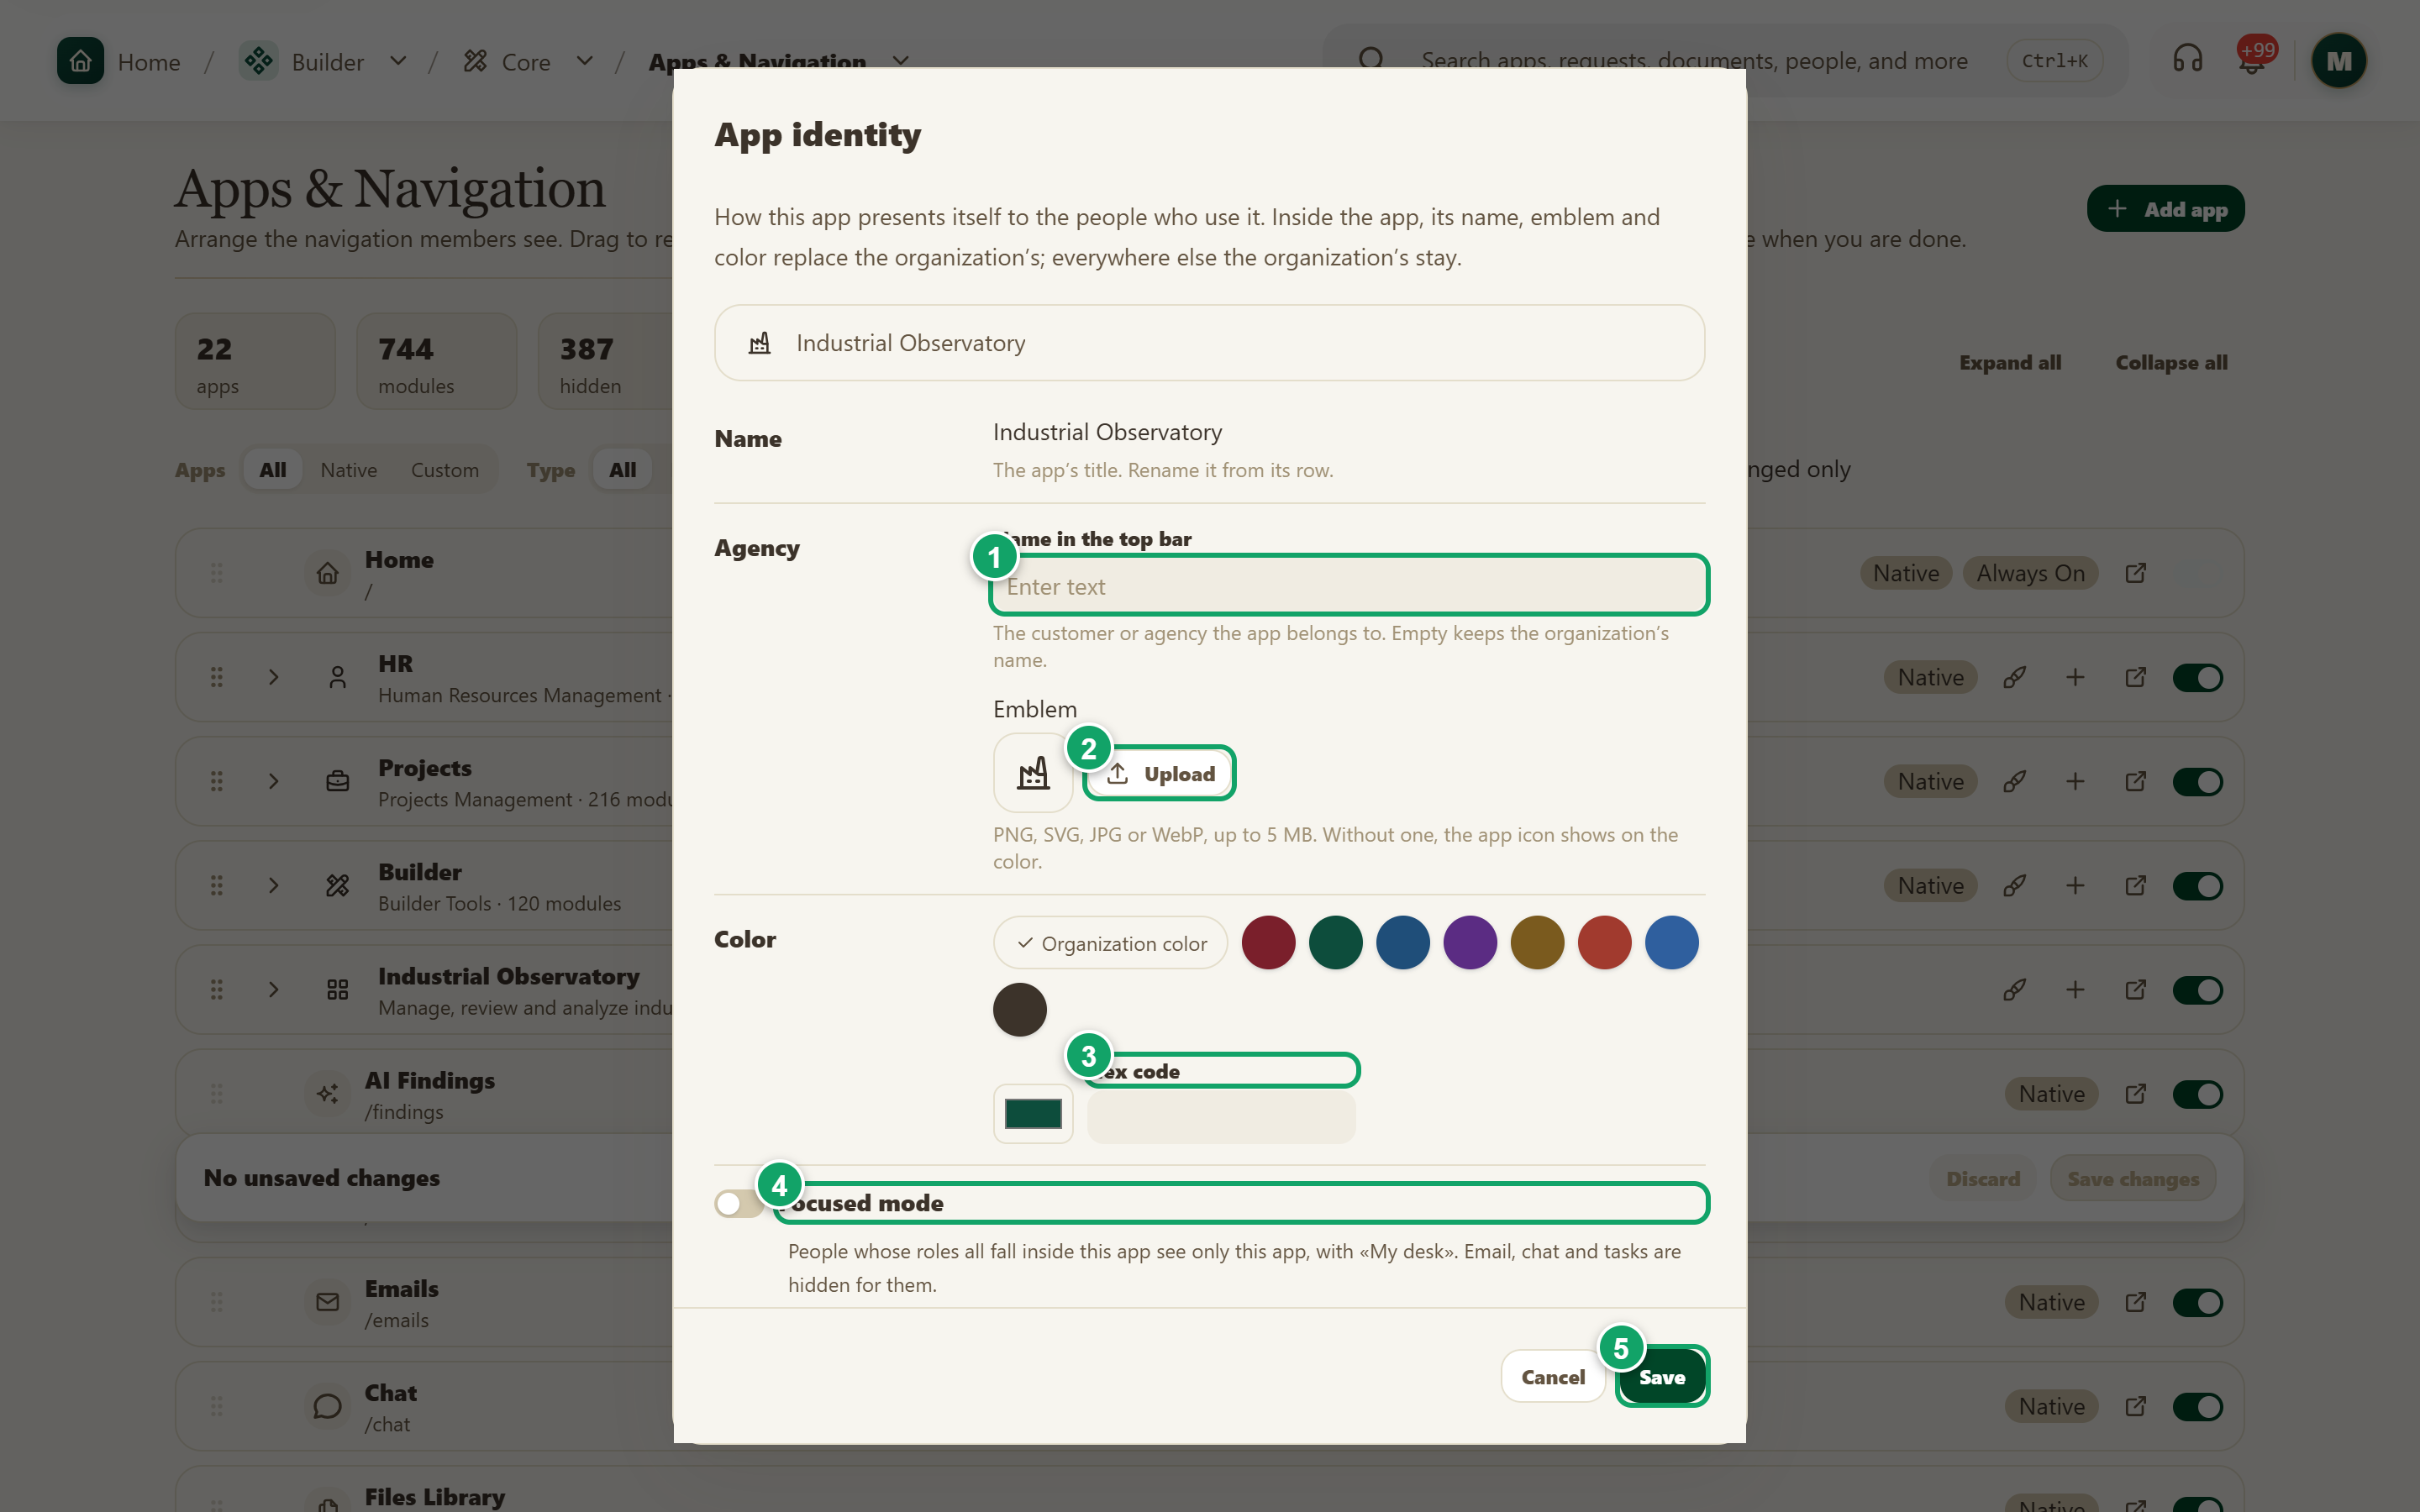
\includegraphics[width=0.95\linewidth,height=0.72\textheight,keepaspectratio]{figures/screens/ch06-nav-identity-en.png}
\caption{The “App identity” dialog}
\label{fig:builder-navigation-identity-screen}
\shotnote{The image shows the “App identity” dialog of the “Industrial Observatory” app in the test organization before any change; it starts with a preview that updates with every choice. The dialog gathers the name, emblem, color and focused mode, and saves them together without “Save changes”. ① “Name in the top bar”: the agency the app belongs to. ② “Upload”: uploads the emblem image. ③ “Hex code”: a custom color in the \en{\#RRGGBB} format; you can pick one of the ready colors instead. ④ “Focused mode”: limits what the app’s members see to this app. ⑤ “Save”: saves the identity at once.}
\end{figure}

\begin{table}[H]
\centering
\caption{What the “App identity” dialog holds}
\label{tab:builder-navigation-identity-fields}
\begin{tabularx}{\linewidth}{R{3.6cm} Y}
\rcHeaderRow
\thh{Part} & \thh{What it sets}\\
Preview & Shows the emblem, color and name together as they will appear in the top bar, and changes with every choice.\\
Name & The app's title, shown only; it is not edited in this dialog.\\
Name in the top bar & The agency or customer the app belongs to, in each language. Left empty, the organization's name stays.\\
Emblem & A \en{PNG}, \en{SVG}, \en{JPG} or \en{WebP} image up to 5 MB, added with “Upload”, changed with “Replace” or removed with “Remove”. Without one, the app icon shows on the color.\\
Color & “Organization color”, one of eight ready colors, or a “Custom color” you pick or type as a “Hex code” in the form \en{\#RRGGBB}. A warning shows if white text is hard to read on the color.\\
Focused mode & People whose roles all fall inside this app see only this app, with «My desk», and Email, chat and tasks are hidden for them. Their permissions stay the same, and administrators always see everything.\\
Keep for them & Shows when focused mode is on; you choose what stays visible for these members: “Tasks”, “Calendar”, “Email”, “Chat”, “Library”, “Form submissions”, “HR” and “Projects”.\\
\end{tabularx}
\end{table}

\begin{rcwarn}[Focused mode only changes what is shown]
Focused mode grants no permission and removes none; it hides the other apps from members whose roles all fall inside this app. A member who has a role in another app is not affected. The tree shows a “Focused” chip next to the app while the mode is on.
\end{rcwarn}

\begin{figure}[H]
\centering
\begin{tikzpicture}[node distance=0.5cm]
\node[stepBox] (a) {App identity button};
\node[stepBox,below=of a] (b) {Name in the top bar};
\node[stepBox,below=of b] (c) {Emblem and color};
\node[stepBox,below=of c] (d) {Focused mode if needed};
\node[stepBox,below=of d] (e) {Review the preview, then save};
\draw[flowsTo] (a) -- (b);
\draw[flowsTo] (b) -- (c);
\draw[flowsTo] (c) -- (d);
\draw[flowsTo] (d) -- (e);
\end{tikzpicture}
\rclegend
\caption{Setting an app's identity}
\label{fig:builder-navigation-identity-flow}
\shotnote{The diagram follows the order of the dialog and puts the preview right before saving, because it shows the result as it will appear in the top bar. The focused-mode step is optional; skip it if the app's members need the other apps in their daily work.}
\end{figure}

\subsection{Steps and check}
\begin{enumerate}
\item Open “Apps \& Navigation”, find the app and press the “App identity” button on its row.
\item Type the “Name in the top bar” if the app belongs to an agency other than the organization.
\item Upload an emblem with “Upload” if you have one, and pick a ready color or type the “Hex code”.
\item Turn on “Focused mode” if the app's members should see only this app, and choose under “Keep for them” what they need.
\item Review the “Preview”, then press “Save”.
\end{enumerate}

\textbf{Check and recovery:} the message “App identity saved.” should appear, and the identity should show in the top bar when the app is opened. If “Save” stays disabled, correct the “Hex code” to the form \en{\#RRGGBB} or clear the field. If “The emblem is larger than 5 MB.” appears, make the image smaller and upload it again.

\clearpage
\section{Add a view to the menu}
\label{sec:builder-feature-navigation-views}

A saved view is a list of records with ready filters and sorting, such as “Requests waiting for review”. You can place it as its own entry in a menu section, so a member opens it directly instead of opening the full list and choosing the filter. It can also show the current number of records, so the member knows the amount of work before opening it.

The view is added as a draft, and members do not see it until you turn its switch on in the tree and save the changes.

\textbf{Path and who uses it:} “Builder” → “Core” → “Apps \& Navigation” → the “Add a view to …” button on the section's row. The button shows when the “Views in menus” feature is on in “Work navigation”, and only for sections that have a record.

\begin{rcnote}[Example: Horizon]
The system administrator adds to the “Visits” section the saved view “Waiting for review” from “Visit requests”, and turns on “Show a live count” with the “Attention” color. Once it is published, Sarah Al-Khatib sees the number of requests waiting for her next to its name in the menu. They pick the type from ①, turn on the count from ③ and choose its colour from ④.
\end{rcnote}

\begin{figure}[H]
\centering
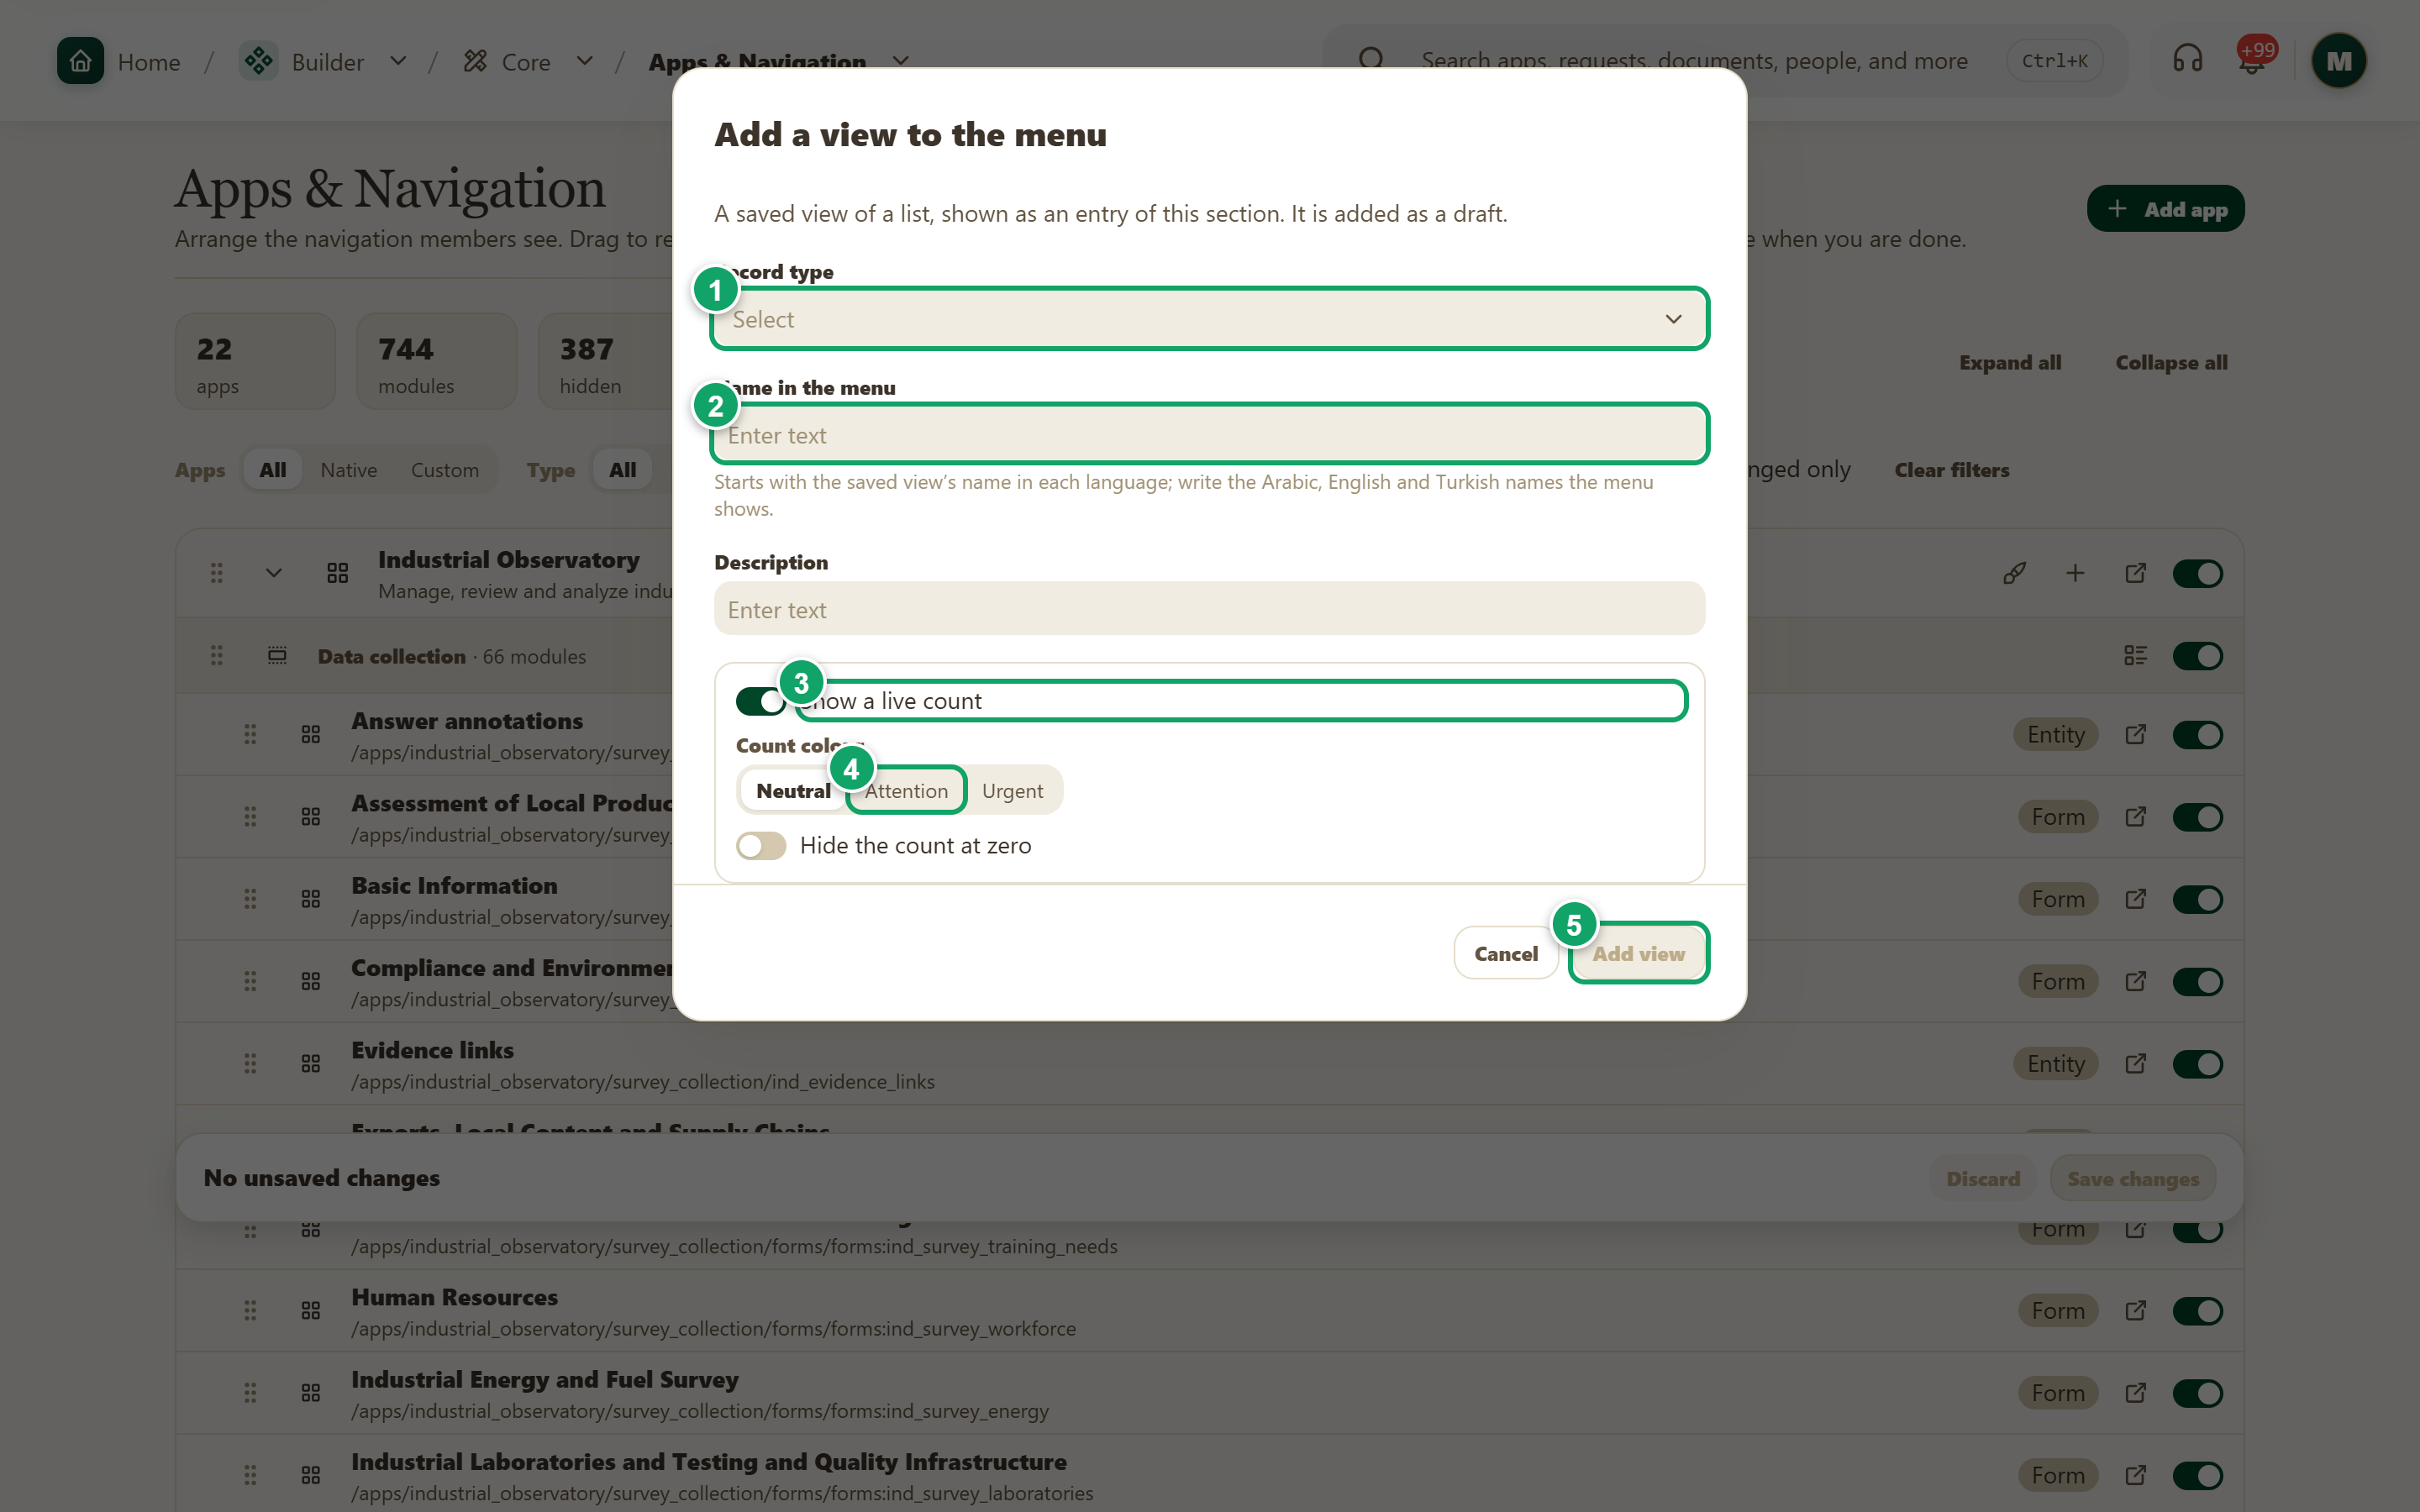
\includegraphics[width=0.95\linewidth,height=0.72\textheight,keepaspectratio]{figures/screens/ch06-nav-add-view-en.png}
\caption{The “Add a view to the menu” dialog}
\label{fig:builder-navigation-views-screen}
\shotnote{The image shows the dialog after pressing the add button in the row of the “Data collection” section in the test organization, before choosing the record type that the list of saved views depends on. “Show a live count” is on by default, and the entry you add stays a draft until you publish it from the tree. ① “Record type”: the type the view comes from. ② “Name in the menu”: the name members see. ③ “Show a live count”: shows the number of records next to the name. ④ “Attention”: one of the count colours. ⑤ “Add view”: adds the entry to the section as a draft.}
\end{figure}

\begin{table}[H]
\centering
\caption{Fields of the “Add a view to the menu” dialog}
\label{tab:builder-navigation-views-fields}
\begin{tabularx}{\linewidth}{R{3.6cm} Y}
\rcHeaderRow
\thh{Field} & \thh{What you choose}\\
Record type & The record type the view comes from. It lists the types the organization built, not the types built into the system.\\
Saved view & One of the type's shared saved views. If it has none, the dialog asks you to add one first in the Builder's “Lists \& views”.\\
Name in the menu & Starts with the view's name, and you can change it in Arabic, English and Turkish.\\
Description & An optional short note on what it shows.\\
Show as & “As the view is saved”, or another layout available for the type, such as a table or board.\\
Show a live count & Shows the number of records next to the name, with a “Count colour”: “Neutral”, “Attention” or “Urgent”, and the option “Hide the count at zero”.\\
\end{tabularx}
\end{table}

\subsection{After adding it}

The new entry shows in the section with a “View” chip and a “Draft” chip. When you turn its switch on and press “Save changes”, it is published and shows for members. To change its name or count later, press the “Edit” button on its row to open “Edit the view in the menu”; saving there keeps the entry published or draft as it was.

\begin{figure}[H]
\centering
\begin{tikzpicture}[node distance=0.5cm]
\node[stepBox] (a) {Turn on Views in menus};
\node[stepBox,below=of a] (b) {Add a view on the section row};
\node[stepBox,below=of b] (c) {Record type and saved view};
\node[stepBox,below=of c] (d) {Name and count};
\node[stepBox,below=of d] (e) {Turn the switch on and save changes};
\draw[flowsTo] (a) -- (b);
\draw[flowsTo] (b) -- (c);
\draw[flowsTo] (c) -- (d);
\draw[flowsTo] (d) -- (e);
\end{tikzpicture}
\rclegend
\caption{From a saved view to a menu entry}
\label{fig:builder-navigation-views-flow}
\shotnote{The diagram starts in “Work navigation” because the add button does not show before the feature is turned on there. It ends with turning the switch on and saving, because adding only creates a draft, and members do not see the entry before it is published.}
\end{figure}

\subsection{Steps and check}
\begin{enumerate}
\item Make sure “Views in menus” is on and saved in “Work navigation”.
\item Open “Apps \& Navigation”, expand the app and press the add-view button on the section's row.
\item Choose the “Record type”, then the “Saved view”, and review the “Name in the menu”.
\item Turn on “Show a live count” if you want it, choose the “Count colour”, then press “Add view”.
\item Turn on the new entry's switch in the section and press “Save changes”.
\end{enumerate}

\textbf{Check and recovery:} after adding, the message “View added to … as a draft” appears with the section's name, and after saving the entry loses its “Draft” chip. If the add button does not show, turn the feature on and save it in “Work navigation”, then reload the page. If the view is missing from the drop-down, make it shared in the Builder's “Lists \& views” and publish the type.

\clearpage
\section{Work navigation}
\label{sec:builder-feature-work-navigation}

This page decides what each member sees first when the day starts, without creating new data. It gathers existing work in places closer to them: a “Due for me” list showing what waits for them, a shared context such as the year or cycle that lists and dashboards follow, and saved views shown in menus with their counts.

The settings are spread over four tabs: “Features”, “Sources”, “Context” and “Dashboards”. They all form one draft saved together with the “Save” button. Every feature is off until you turn it on, and an organization that turns none on behaves exactly as before.

\textbf{Path and who uses it:} “Builder” → “Core” → “Work navigation”. Available only to the organization owner and administrator.

\begin{rcnote}[Example: Horizon]
The system administrator turns on “Due for me” and adds to it the visit requests waiting for Sarah Al-Khatib's decision, so Sarah finds them in one place every morning instead of opening each list. They turn on the feature from ② in tab ①, then add the source from ③ and save from ④.
\end{rcnote}

\begin{figure}[H]
\centering
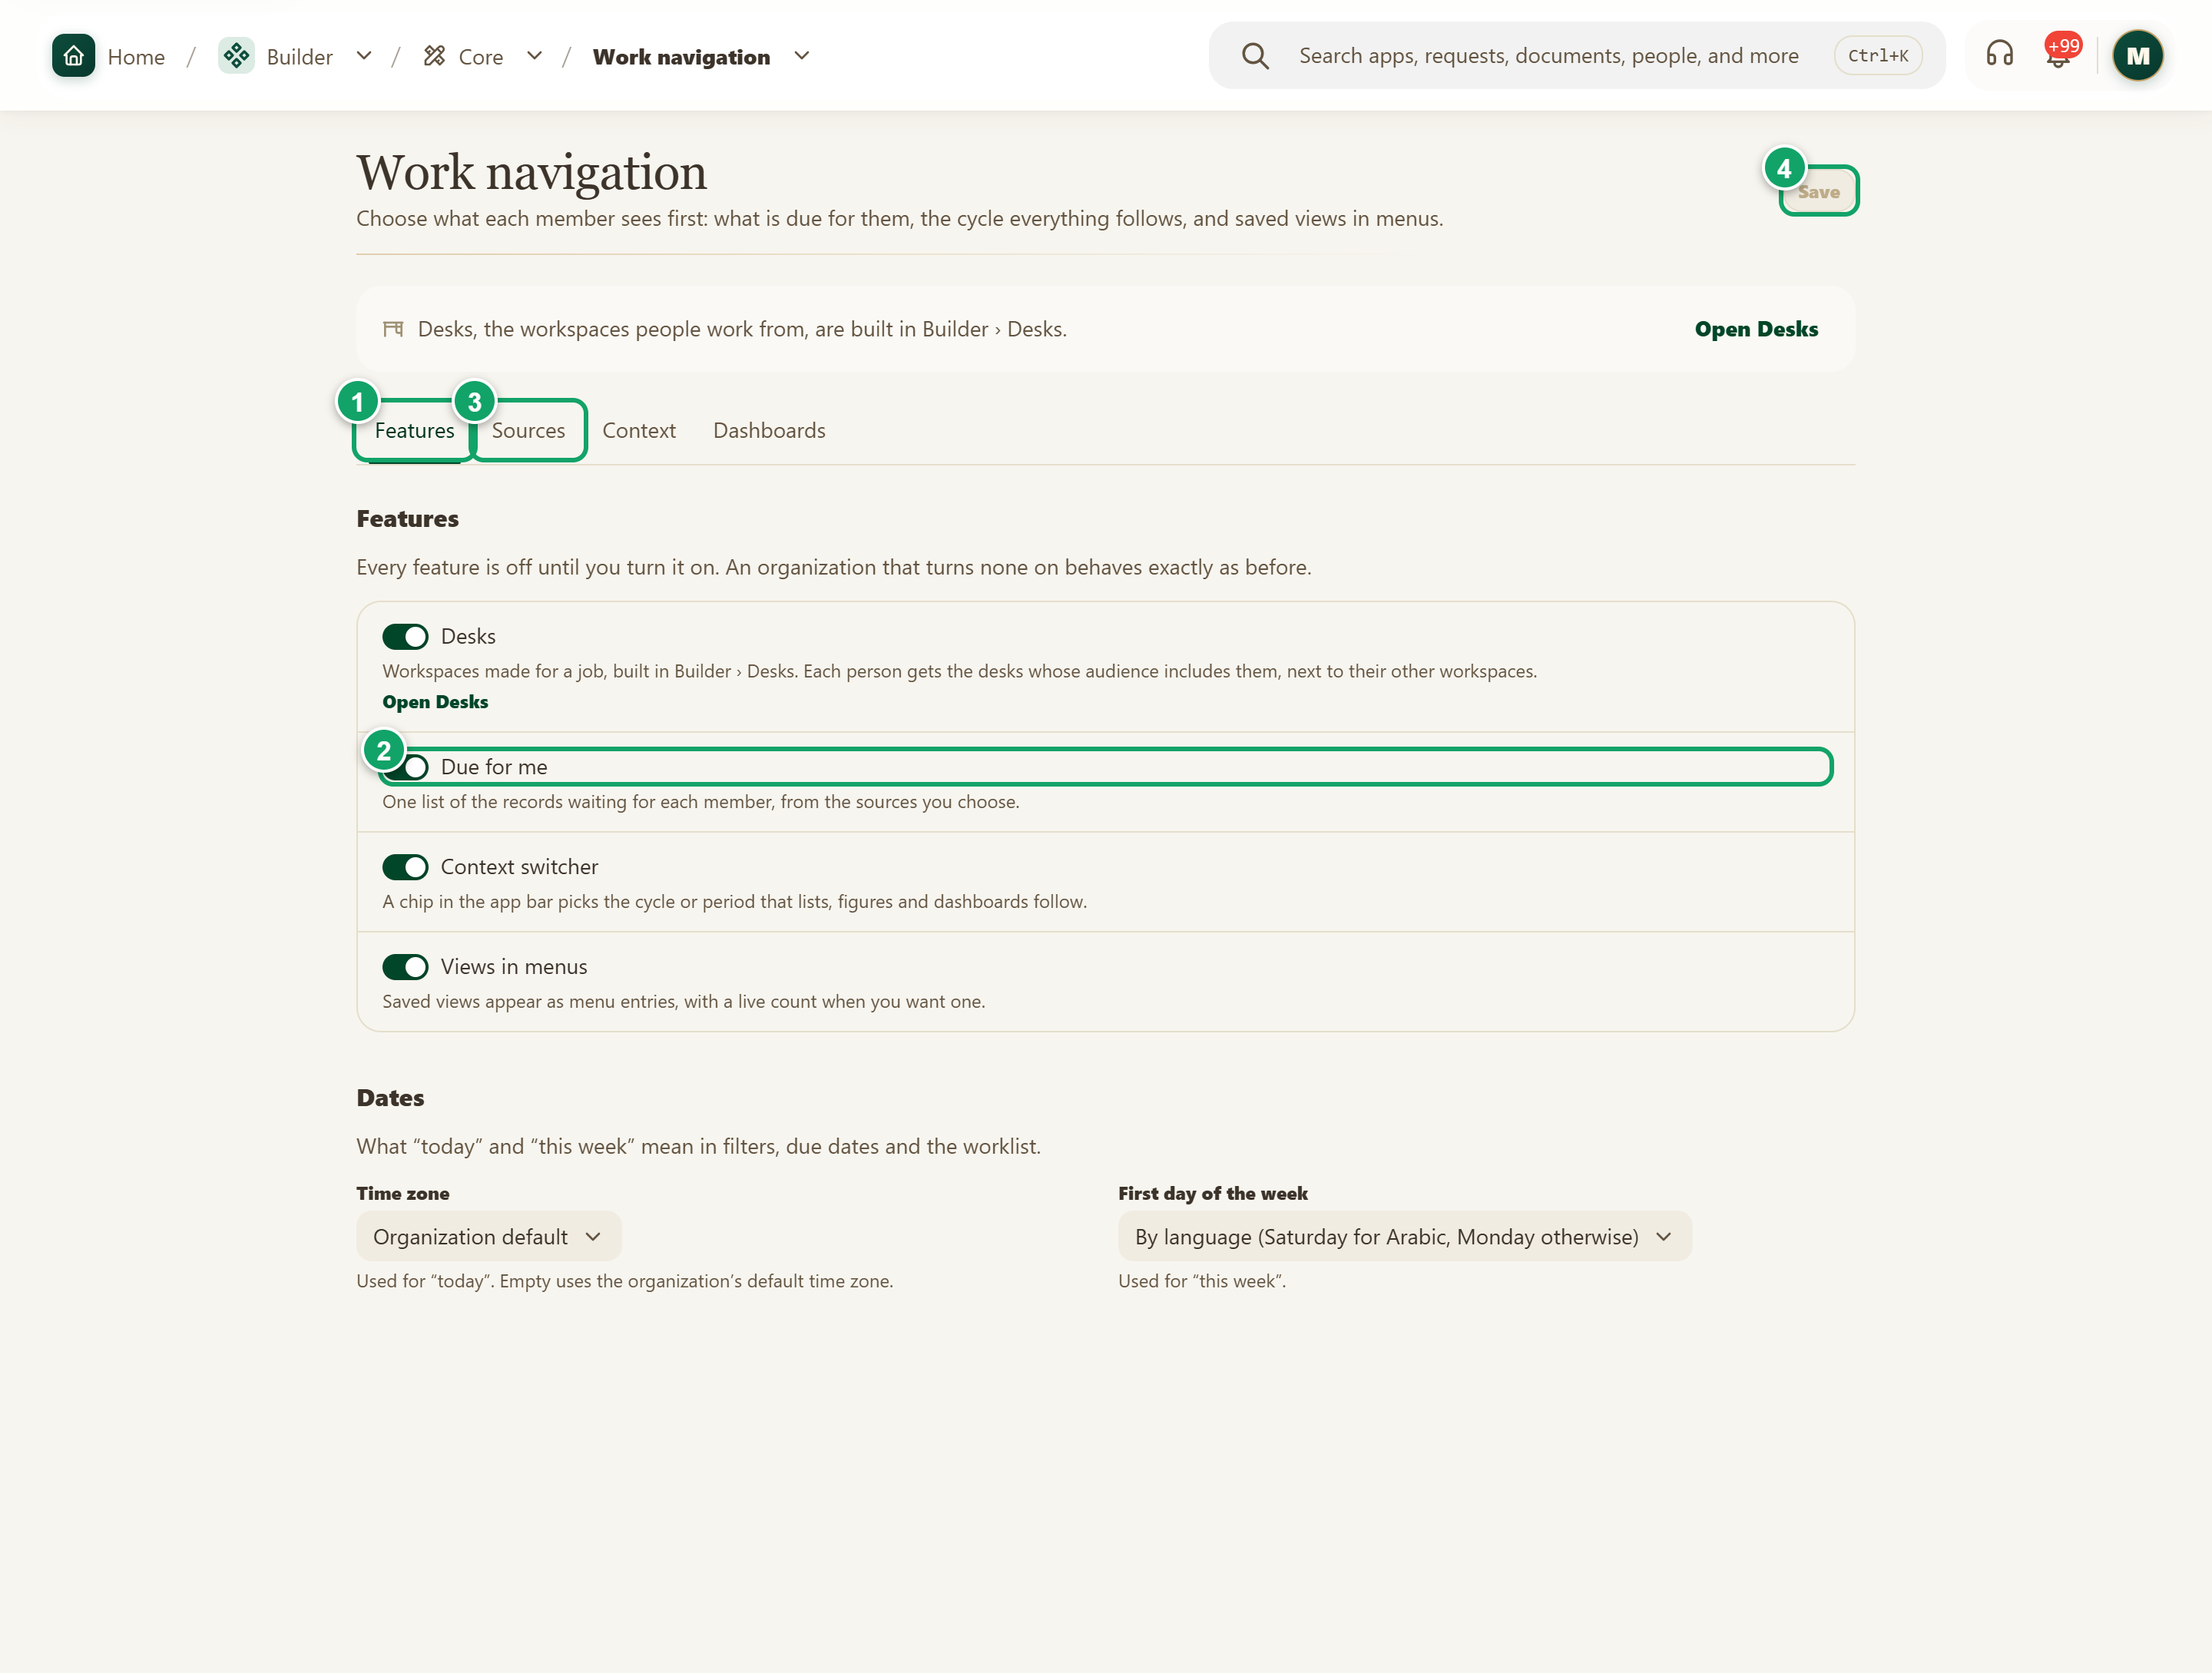
\includegraphics[width=0.95\linewidth,height=0.72\textheight,keepaspectratio]{figures/screens/ch06-work-navigation-en.png}
\caption{The “Work navigation” page}
\label{fig:builder-work-navigation-screen}
\shotnote{The image shows the “Features” tab in the test organization, where all four features are on; in an organization that has not set up the page, they all start off. The four tabs are saved together with one button, so review what you changed in them before saving. ① “Features”: the tab where you turn on “Desks”, “Due for me” and more. ② The “Due for me” switch: turns on the list gathering what waits for the member. ③ “Sources”: sets what feeds this list. ④ “Save”: saves the settings and stays disabled until you change something.}
\end{figure}

\begin{table}[H]
\centering
\caption{The “Features” tab}
\label{tab:builder-work-navigation-data}
\begin{tabularx}{\linewidth}{R{3.6cm} Y}
\rcHeaderRow
\thh{Setting} & \thh{What does it do?}\\
Desks & Turns on desks, workspaces made for a job. Desks are built on a separate page you open from the “Open Desks” link.\\
Due for me & Gathers in one list the records waiting for each member, from the sources you add in the “Sources” tab.\\
Context switcher & Shows a chip in the app bar from which a member picks the cycle or period that lists, figures and dashboards follow.\\
Views in menus & Lets saved views appear as menu entries, with their live count when wanted.\\
Dates & The “Time zone” used for “today” and the “First day of the week” used for “this week”, in filters, due dates and the due list.\\
\end{tabularx}
\end{table}

\begin{table}[H]
\centering
\caption{The other tabs}
\label{tab:builder-work-navigation-tabs}
\begin{tabularx}{\linewidth}{R{3.6cm} Y}
\rcHeaderRow
\thh{Tab} & \thh{What do you set there?}\\
Sources & What feeds the “Due for me” list. Explained in “Due for me sources”.\\
Context & The record type that chosen apps and sections follow. Explained in “Context”.\\
Dashboards & The data scope of new dashboards, and moving older dashboards to the viewer's permissions. Explained in “Dashboard data scope”.\\
\end{tabularx}
\end{table}

\begin{figure}[H]
\centering
\begin{tikzpicture}[node distance=0.5cm]
\node[entity] (member) {Member};
\node[entityOpt,below right=0.7cm and 0.3cm of member] (desk) {Desks};
\node[entityOpt,below left=0.7cm and 0.3cm of member] (due) {Due for me};
\draw[dependsOnOpt] (member.south) -- ++(0,-0.3) -| (desk.north);
\draw[dependsOnOpt] (member.south) -- ++(0,-0.3) -| (due.north);
\end{tikzpicture}
\rclegend
\caption{What the member sees first}
\label{fig:builder-work-navigation-model}
\shotnote{The figure shows that this page creates no new data; it brings existing work closer to the member: desks that suit their job, and a list gathering what is due for them across record types. Both are optional, so turn on one feature and try it before turning on others.}
\end{figure}

\subsection{Steps and check}
\begin{enumerate}
\item Open “Work navigation” and turn on, under “Features”, the feature the organization needs.
\item Choose the “Time zone” and “First day of the week” if the defaults do not suit the organization.
\item If you turned on “Due for me”, go to “Sources” and add at least one source.
\item Press “Save” in the page header, or “Discard changes” to undo everything you have not saved.
\end{enumerate}

\textbf{Check and recovery:} the message “Work navigation saved” should appear, and “Save” should become disabled until you change something else. If the note “Add at least one source in Sources, or the list stays empty.” shows under “Due for me”, add a source before telling members about the feature. If “Settings that need attention” or a save conflict appears, follow “Settings that need attention”.

\clearpage
\section{Due for me sources}
\label{sec:builder-feature-work-navigation-sources}

The “Due for me” list starts empty and shows only what its sources define. A source is a rule that says: show the member these records because they wait for them. They may be records on which the member can run a transition now, records assigned to them in a member field, or a list built into the system, such as approvals.

Each source adds its records to the lists of every member who meets its conditions, and it can be limited to certain roles. A source grants no new permission: a member sees only records they can open.

\textbf{Path and who uses it:} “Builder” → “Core” → “Work navigation” → “Sources”. Used by the organization owner and administrator after turning on “Due for me”.

\begin{rcnote}[Example: Horizon]
The system administrator adds a “Transitions I can run” source named “Visits awaiting a decision”, choosing “Visit requests”, its status field and the approval transition. The requests then show in Sarah Al-Khatib's list because she can approve them, and not in Omar Haddad's. They add the source from ②, save from ③ and check it from ④.
\end{rcnote}

\begin{figure}[H]
\centering
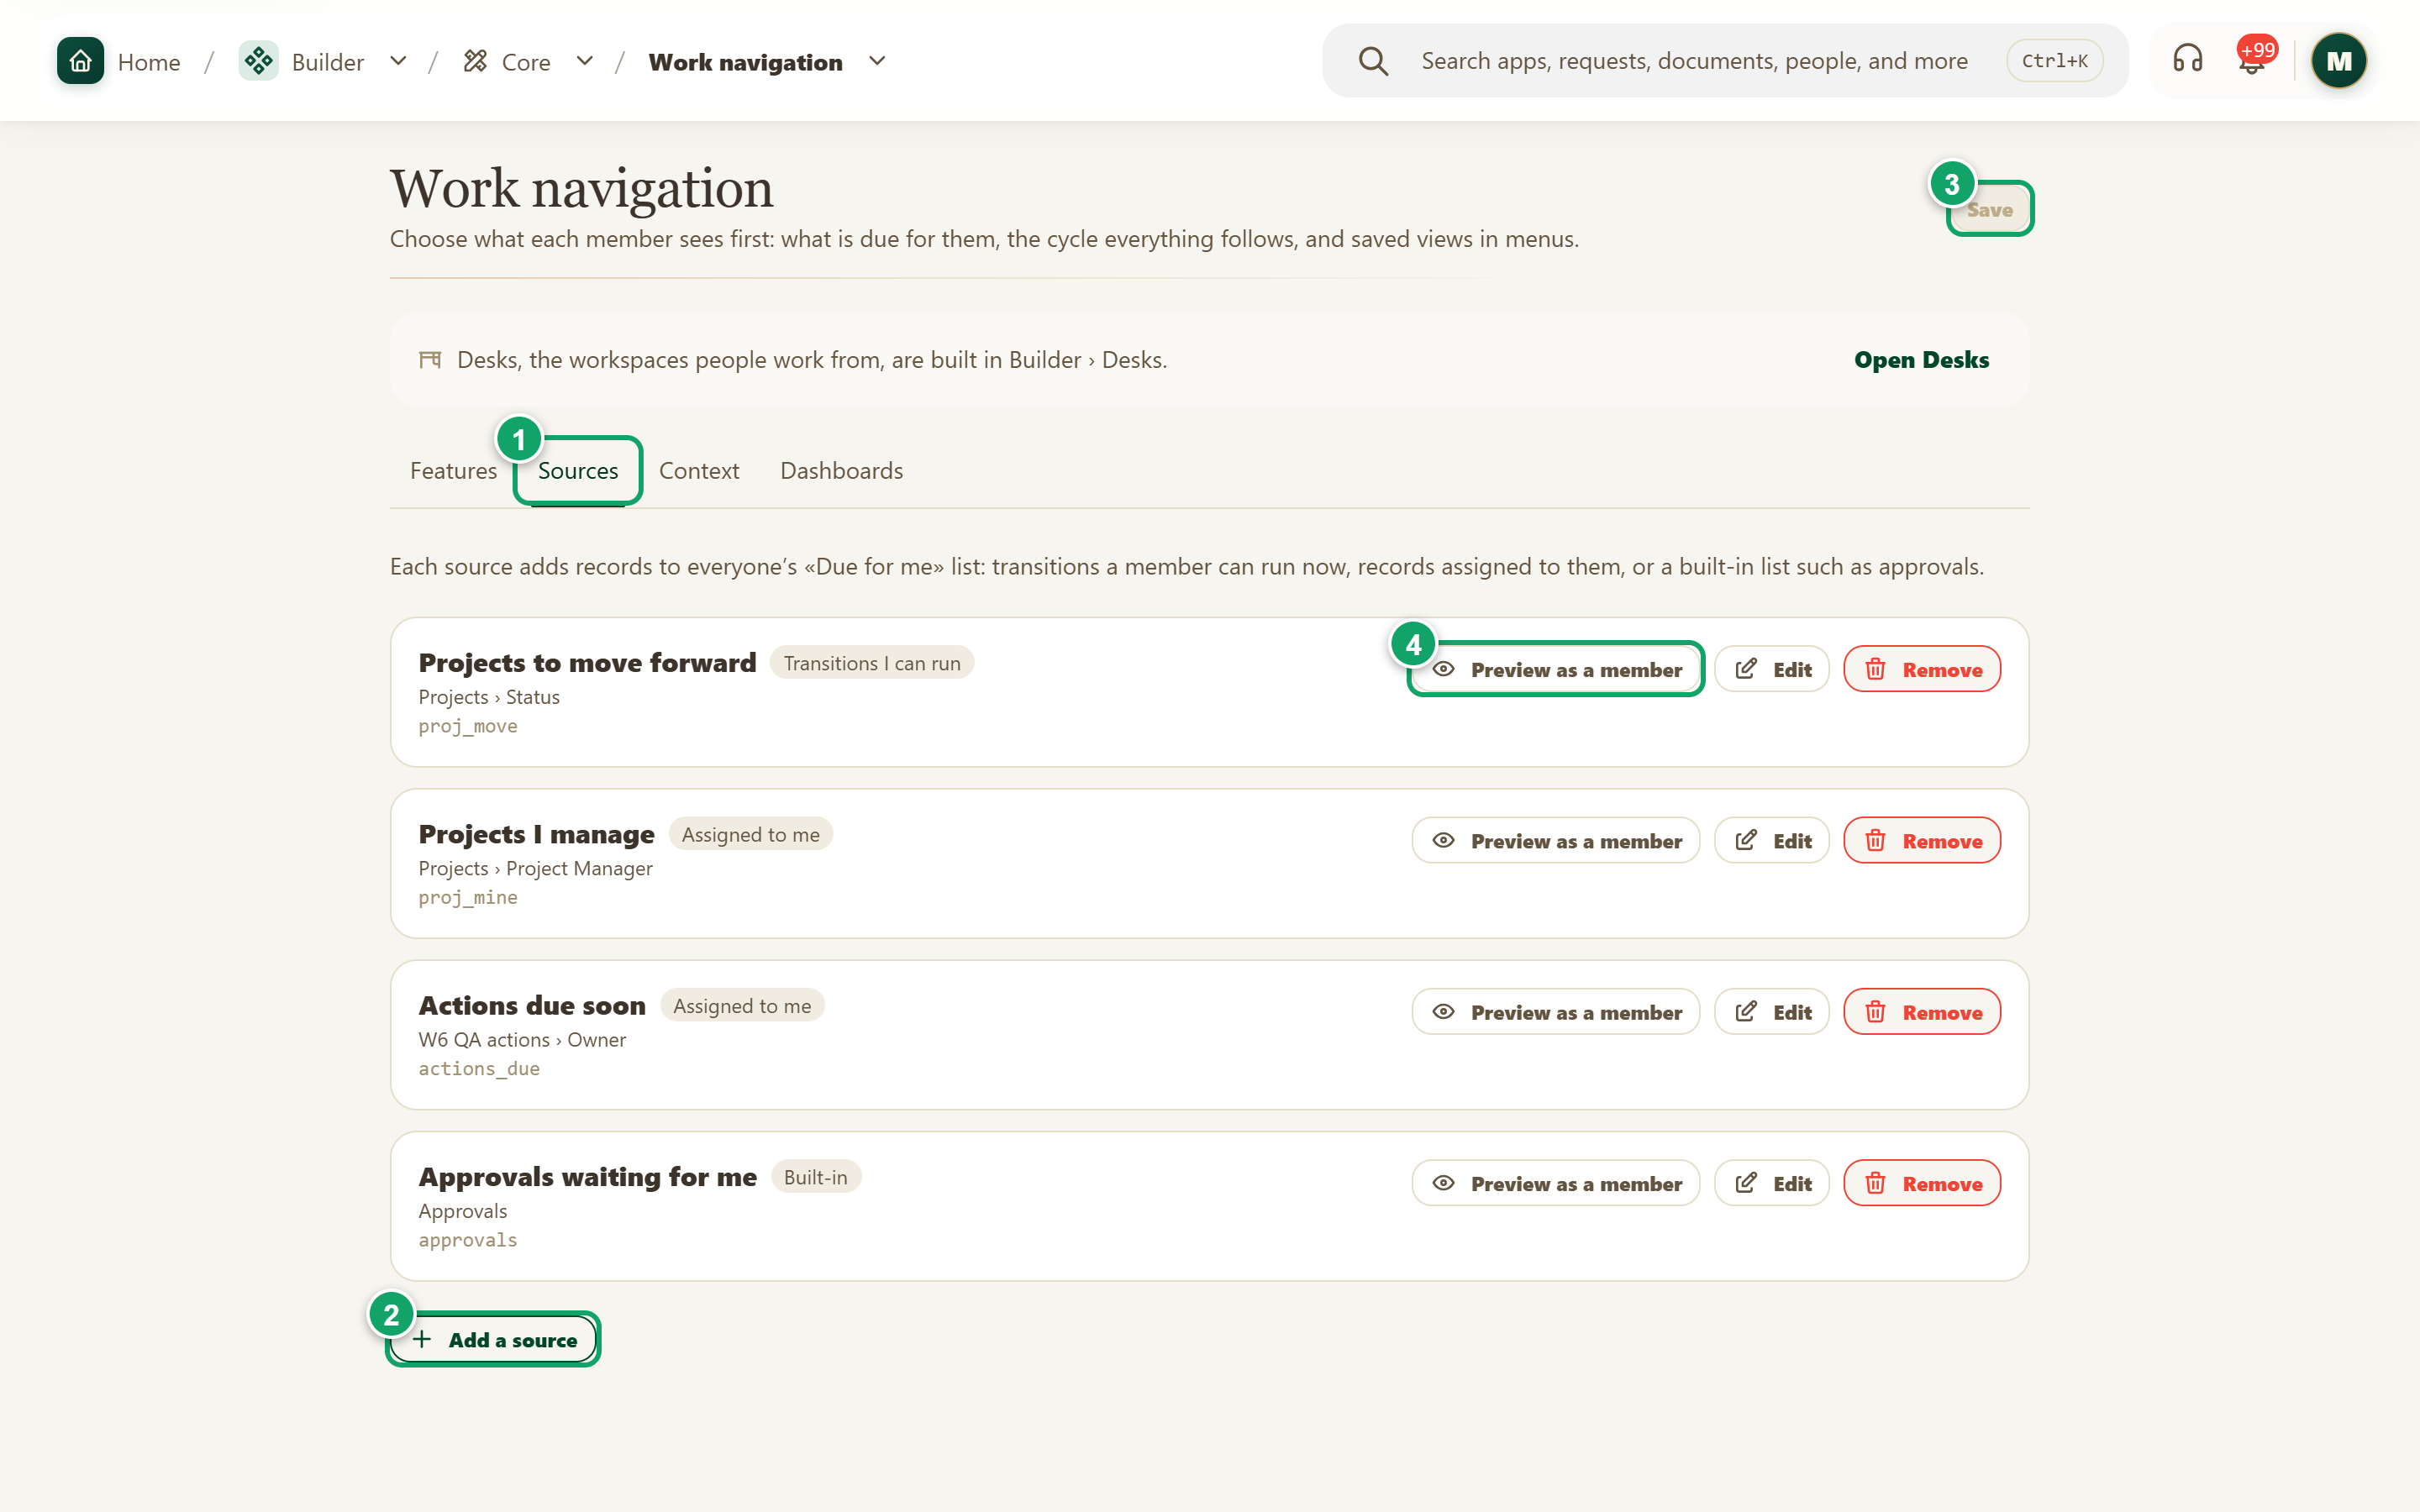
\includegraphics[width=0.95\linewidth,height=0.72\textheight,keepaspectratio]{figures/screens/ch06-wn-sources-en.png}
\caption{The “Sources” tab}
\label{fig:builder-work-navigation-sources-screen}
\shotnote{The image shows the “Sources” tab in the test organization, with four sources of the three kinds; each carries its kind’s chip, the record type it reads and its key. It helps you compare the existing sources before adding a new one. ① “Sources”: the tab that lists the sources. ② “Add a source”: opens the new source dialog. ③ “Save”: saves the sources with the rest of the page. ④ “Preview as a member”: shows the record count and examples after saving.}
\end{figure}

\begin{table}[H]
\centering
\caption{Kinds of source}
\label{tab:builder-work-navigation-sources-kinds}
\begin{tabularx}{\linewidth}{R{3.6cm} Y}
\rcHeaderRow
\thh{Kind} & \thh{What it brings and what you set}\\
Transitions I can run & Records on which the member can run a transition now, such as approving or reviewing. You choose the “Record type”, the “Status field” and the “Transitions that count as work”; left empty, it covers every transition except plain editing.\\
Assigned to me & Records where one of the “Member fields” names the member. You can set “Which statuses are open”: “Any status”, “By category” or “Chosen statuses”, and set a window with “Starts on (field)” and “Ends on (field)”.\\
Built-in & A ready list you pick under “Built-in list”, such as “Approvals”, “SOP approvals”, “Tasks”, “Task requests” and “Cycles”.\\
\end{tabularx}
\end{table}

\begin{table}[H]
\centering
\caption{Shared settings in the source dialog}
\label{tab:builder-work-navigation-sources-common}
\begin{tabularx}{\linewidth}{R{3.6cm} Y}
\rcHeaderRow
\thh{Setting} & \thh{What it sets}\\
What the rows are to the person & “Work to do”, “Following” or “Waiting on others”. Assigned records that wait on others also get “Late after (days)”.\\
Name and key & The “Name” is shown to members, and the “Key” is an identifier of Latin letters, digits and underscores that cannot change after the source is added.\\
Due dates & The “Due date field”, and “Due within (days)” to show overdue records and those due soon.\\
Row display & “Row title” and “Row subtitle”, and “Open this related record” so the row opens another record the field points at.\\
Roles and priority & “Roles that see it”; left empty, everyone who can open the records sees it. “Priority”: sources with a lower number come first.\\
Extra filters (advanced) & Extra conditions in \en{JSON} for those who need finer filtering.\\
\end{tabularx}
\end{table}

\begin{figure}[H]
\centering
\begin{tikzpicture}[node distance=0.5cm]
\node[stepBox] (a) {Add a source};
\node[stepBox,below=of a] (b) {Kind and meaning of the rows};
\node[stepBox,below=of b] (c) {Record type and fields};
\node[stepBox,below=of c] (d) {Roles and priority};
\node[stepBox,below=of d] (e) {Save the page};
\node[stepBox,below=of e] (f) {Preview as a member};
\draw[flowsTo] (a) -- (b);
\draw[flowsTo] (b) -- (c);
\draw[flowsTo] (c) -- (d);
\draw[flowsTo] (d) -- (e);
\draw[flowsTo] (e) -- (f);
\end{tikzpicture}
\rclegend
\caption{Adding and trying a source}
\label{fig:builder-work-navigation-sources-flow}
\shotnote{The diagram puts the preview after saving because it reads only the saved settings, so it shows nothing for a source not saved yet. The dialog's button adds the source to the draft, which is why “Save” in the page header is still needed.}
\end{figure}

\subsection{Steps and check}
\begin{enumerate}
\item Open “Work navigation”, then the “Sources” tab, and press “Add a source”.
\item Choose the “Kind” and “What the rows are to the person”, and enter the “Name” and “Key”.
\item Choose the “Record type” and the fields the kind asks for, and set “Roles that see it” if needed.
\item Press “Add a source” in the dialog, then “Save” in the page header.
\item Press “Preview as a member” on the source's row to see the number of records and some examples with your own permissions.
\end{enumerate}

\textbf{Check and recovery:} the source should show in the list, and the preview should show a count after saving. If the dialog's button stays disabled, read the messages under it, such as “Choose a record type.” or “Another source already uses this key.”. If the preview says “You hold none of this source’s roles, so there is nothing to preview as you.”, the source is correct but meant for roles you do not hold. The tab holds at most twenty sources.

\clearpage
\section{Context}
\label{sec:builder-feature-work-navigation-context}

A context is a record type, such as a cycle or a year, that the lists, figures and dashboards of chosen apps and sections follow. A member picks the context value once from a chip in the app bar, and every page of those apps then shows only what belongs to that value. This saves the member from repeating the same filter in every list.

The chip shows for members only after “Context switcher” is turned on under “Features”. At most three contexts can be defined.

\textbf{Path and who uses it:} “Builder” → “Core” → “Work navigation” → “Context”. Used by the organization owner and administrator when work is organized in cycles or periods.

\begin{rcnote}[Example: Horizon]
Horizon organizes its visits in quarterly cycles. The system administrator adds a context on the cycles record type, makes the “Branch services” app follow it, and picks the relation of “Visit requests” to the cycle. When Sarah Al-Khatib picks the current cycle, she sees only its requests. They pick the record type from ② and the app from ④.
\end{rcnote}

\begin{figure}[H]
\centering
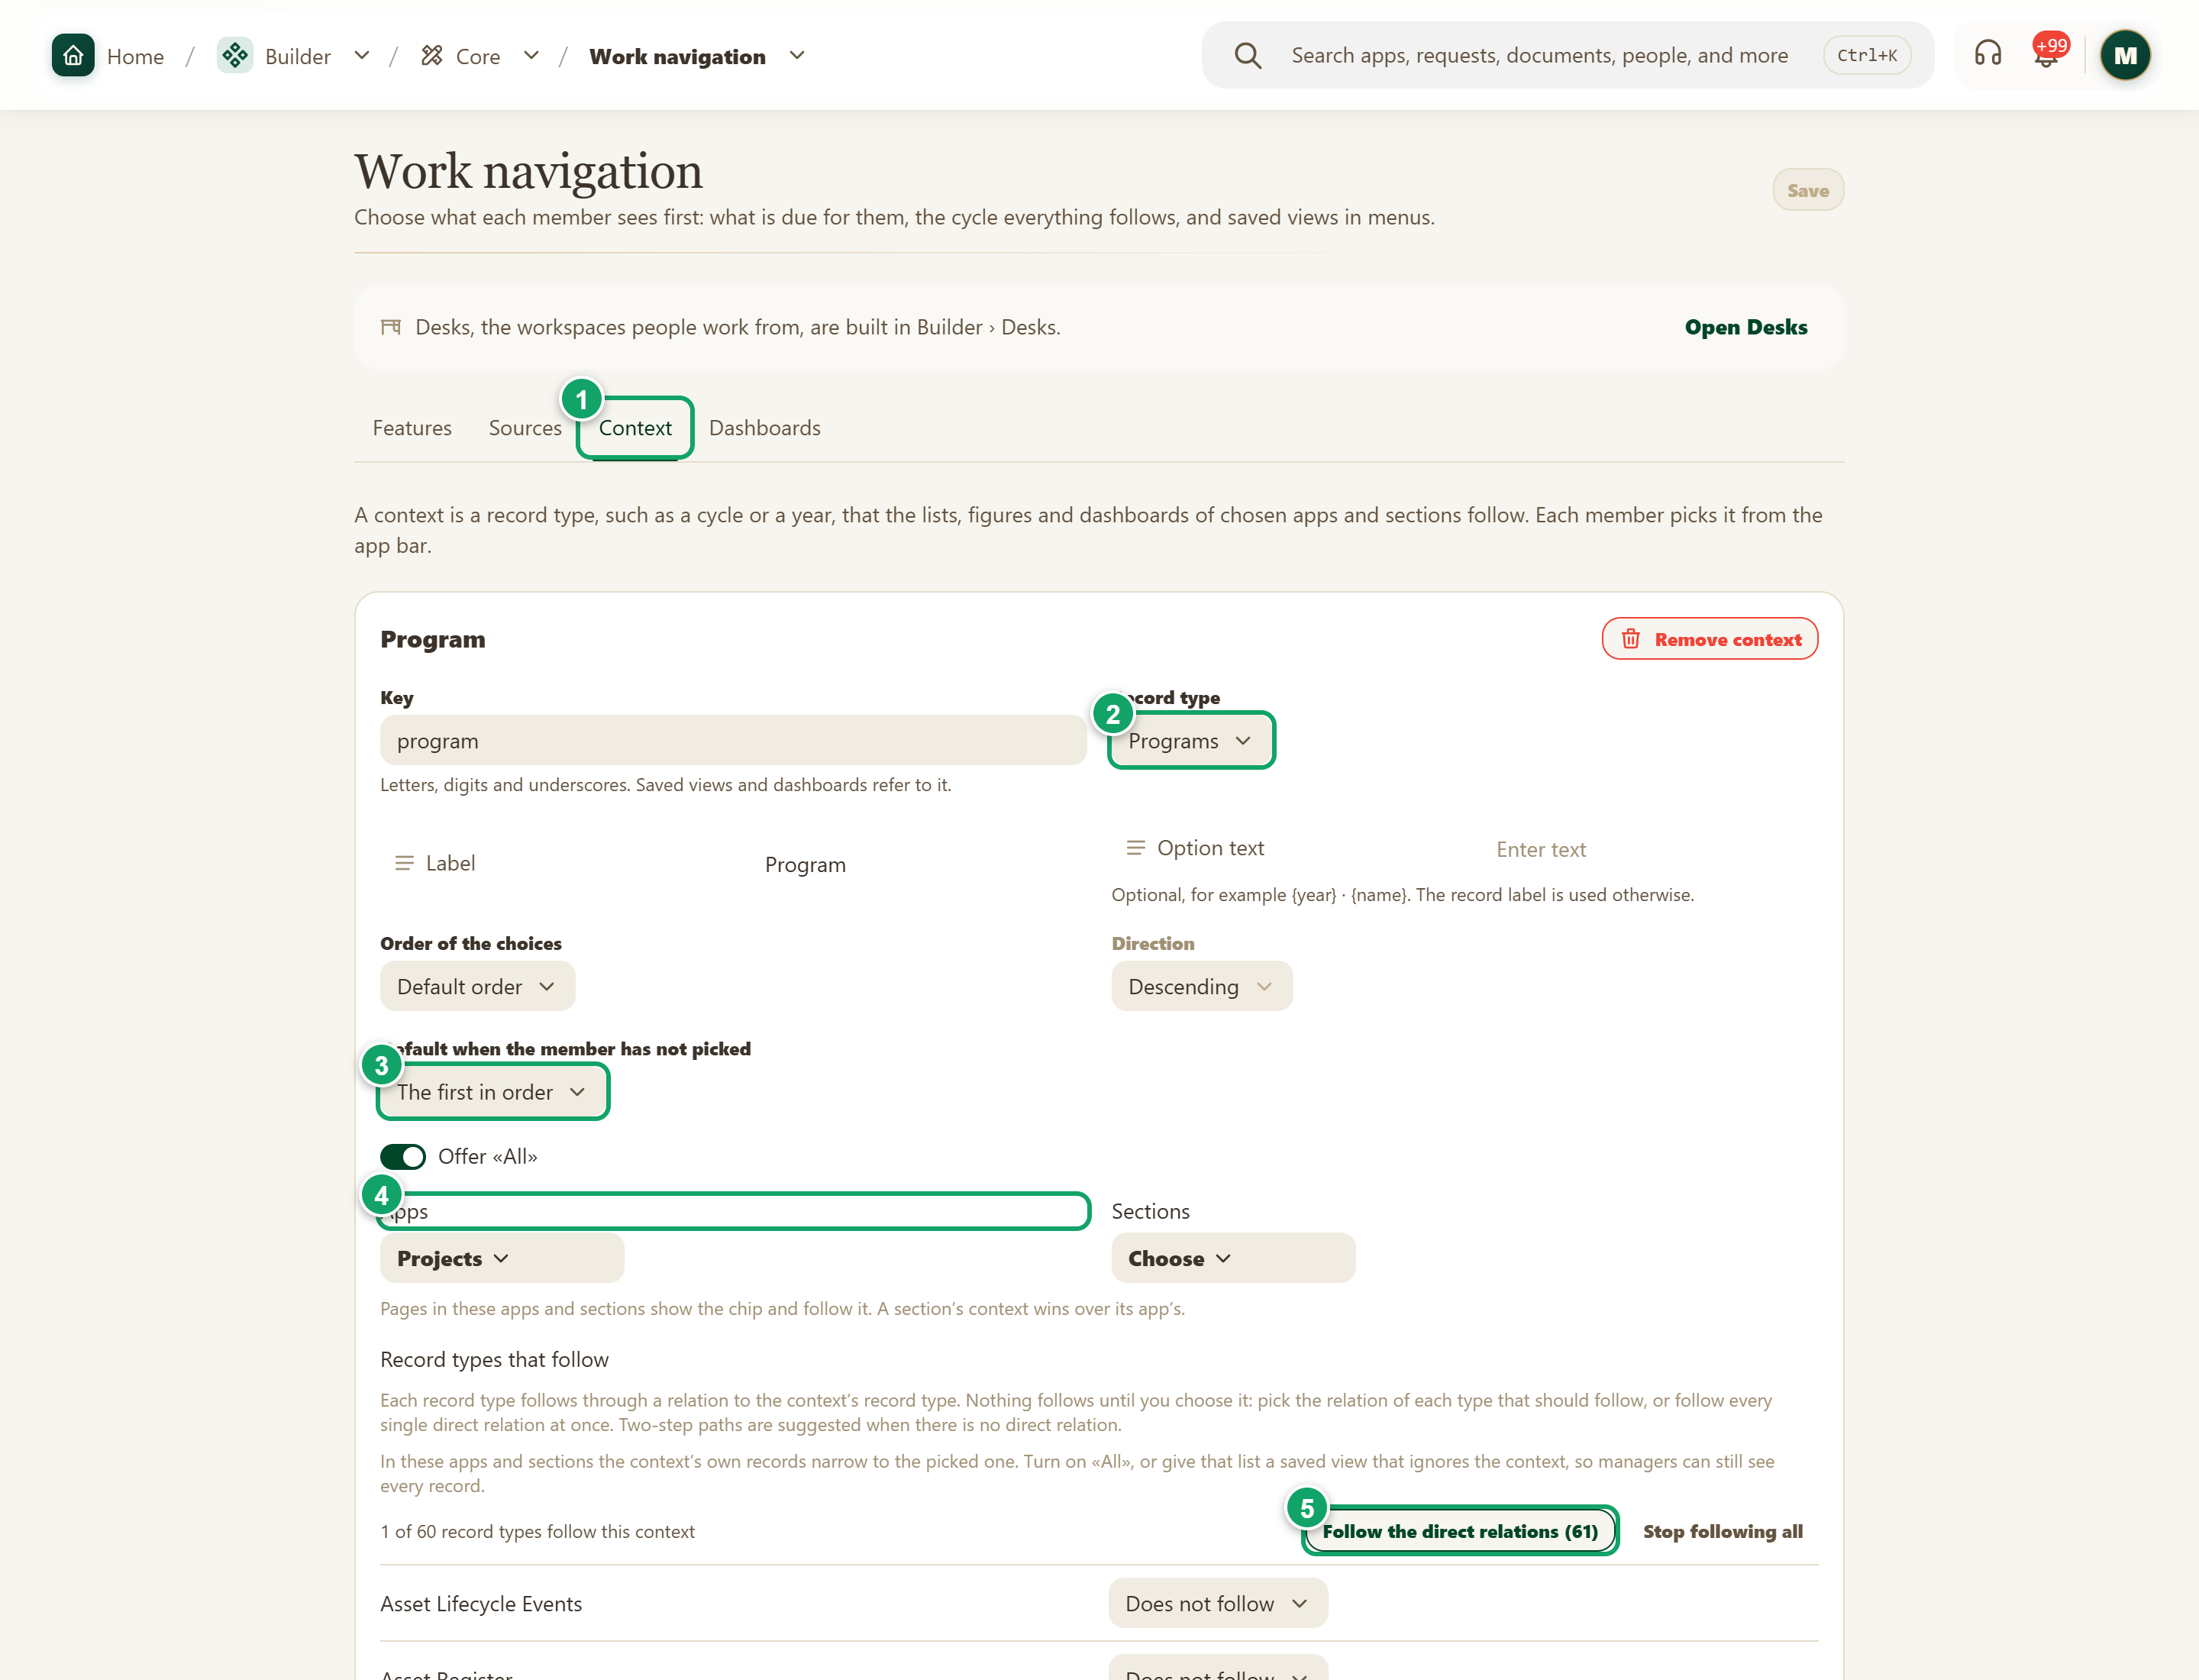
\includegraphics[width=0.95\linewidth,height=0.72\textheight,keepaspectratio]{figures/screens/ch06-wn-context-en.png}
\caption{The “Context” tab}
\label{fig:builder-work-navigation-context-screen}
\shotnote{The image shows the “Context” tab in the test organization, with a context called “Program” built on the “Programs” record type and followed by the “Projects” app. Below it, the “Record types that follow” table shows most types on “Does not follow”, because following does not start until you choose it. ① “Context”: the tab where you set contexts. ② “Record type”: the cycles or years type the context is built on. ③ “Default when the member has not picked”: the value shown before the member picks. ④ “Apps”: the places that show the chip and follow it, next to “Sections”. ⑤ “Follow the direct relations”: picks every single direct relation at once.}
\end{figure}

\begin{table}[H]
\centering
\caption{Context settings}
\label{tab:builder-work-navigation-context-fields}
\begin{tabularx}{\linewidth}{R{3.6cm} Y}
\rcHeaderRow
\thh{Setting} & \thh{What it sets}\\
Key, record type and label & The “Key” is an identifier that saved views and dashboards refer to, the “Record type” is the cycles or years type, and the “Label” is what the member sees.\\
Option text & An optional pattern for the text of each option in the chip. Left empty, the record label is used.\\
Order of the choices and direction & The field the options are sorted by, and “Ascending” or “Descending”.\\
Default when the member has not picked & “The first in order”, “The first in a status” with a “Status field” and “Statuses”, or “Nothing (show all)”.\\
Offer «All» & Adds an option to the chip that shows every record without narrowing.\\
Apps and sections & The places that show the chip and follow it. A section's context wins over its app's.\\
Record types that follow & For each record type you choose under “Follows through” the relation it follows the context by, or choose “Does not follow”. The “Follow the direct relations” button picks every single direct relation at once.\\
\end{tabularx}
\end{table}

\begin{rcwarn}[Nothing follows until you choose it]
Adding an app to the context is not enough on its own; a record type narrows only after you choose a relation for it under “Record types that follow”. Also, the context's own records narrow to the picked value in those places, so turn on «All» so administrators can still see every record.
\end{rcwarn}

\begin{figure}[H]
\centering
\begin{tikzpicture}[node distance=0.5cm]
\node[stepBox] (a) {Turn on Context switcher};
\node[stepBox,below=of a] (b) {Add context};
\node[stepBox,below=of b] (c) {Record type and default};
\node[stepBox,below=of c] (d) {Apps and sections};
\node[stepBox,below=of d] (e) {Record types that follow};
\node[stepBox,below=of e] (f) {Save};
\draw[flowsTo] (a) -- (b);
\draw[flowsTo] (b) -- (c);
\draw[flowsTo] (c) -- (d);
\draw[flowsTo] (d) -- (e);
\draw[flowsTo] (e) -- (f);
\end{tikzpicture}
\rclegend
\caption{Setting a shared context}
\label{fig:builder-work-navigation-context-flow}
\shotnote{The diagram starts by turning the feature on because the chip does not show for members without it, even when the context is set. It puts the following record types after the places, because the place decides where the chip shows, while the relation decides which records actually narrow.}
\end{figure}

\subsection{Steps and check}
\begin{enumerate}
\item Turn on “Context switcher” in the “Features” tab.
\item Open the “Context” tab and press “Add context”, then enter the “Key”, choose the “Record type” and enter the “Label”.
\item Choose the “Default when the member has not picked”, and turn on “Offer «All»” if needed.
\item Choose the “Apps” and “Sections” that follow it, then choose for each record type the relation it follows through.
\item Press “Save” in the page header.
\end{enumerate}

\textbf{Check and recovery:} after saving and reloading the page, the chip shows in the bar of the chosen apps, and their lists narrow when a value is picked. If a list does not narrow, go back to “Record types that follow” and make sure its type is not set to “Does not follow”. If “Already follows «…»” shows next to an app, it follows another context, so remove it from that context first.

\clearpage
\section{Dashboard data scope}
\label{sec:builder-feature-work-navigation-dashboards}

A dashboard shows numbers and charts calculated from records. Its “data scope” decides which records they come from: either “With the viewer’s permissions”, so each person sees numbers from the records they may see, or “All organization data”, so everyone who opens the dashboard sees the numbers of all records.

This tab sets two things: the scope new dashboards are created with, and the list of existing dashboards that still show organization-wide data, which you can switch to the viewer's permissions.

\textbf{Path and who uses it:} “Builder” → “Core” → “Work navigation” → “Dashboards”. Only organization owners and administrators see the list of dashboards.

\begin{rcnote}[Example: Horizon]
The system administrator finds in the list the visits dashboard that shows both branches' numbers to everyone who opens it. They switch it to the viewer's permissions, so Omar Haddad sees only his own requests' numbers, while Sarah Al-Khatib sees what her permissions allow. They switch the dashboard from ④.
\end{rcnote}

\begin{figure}[H]
\centering
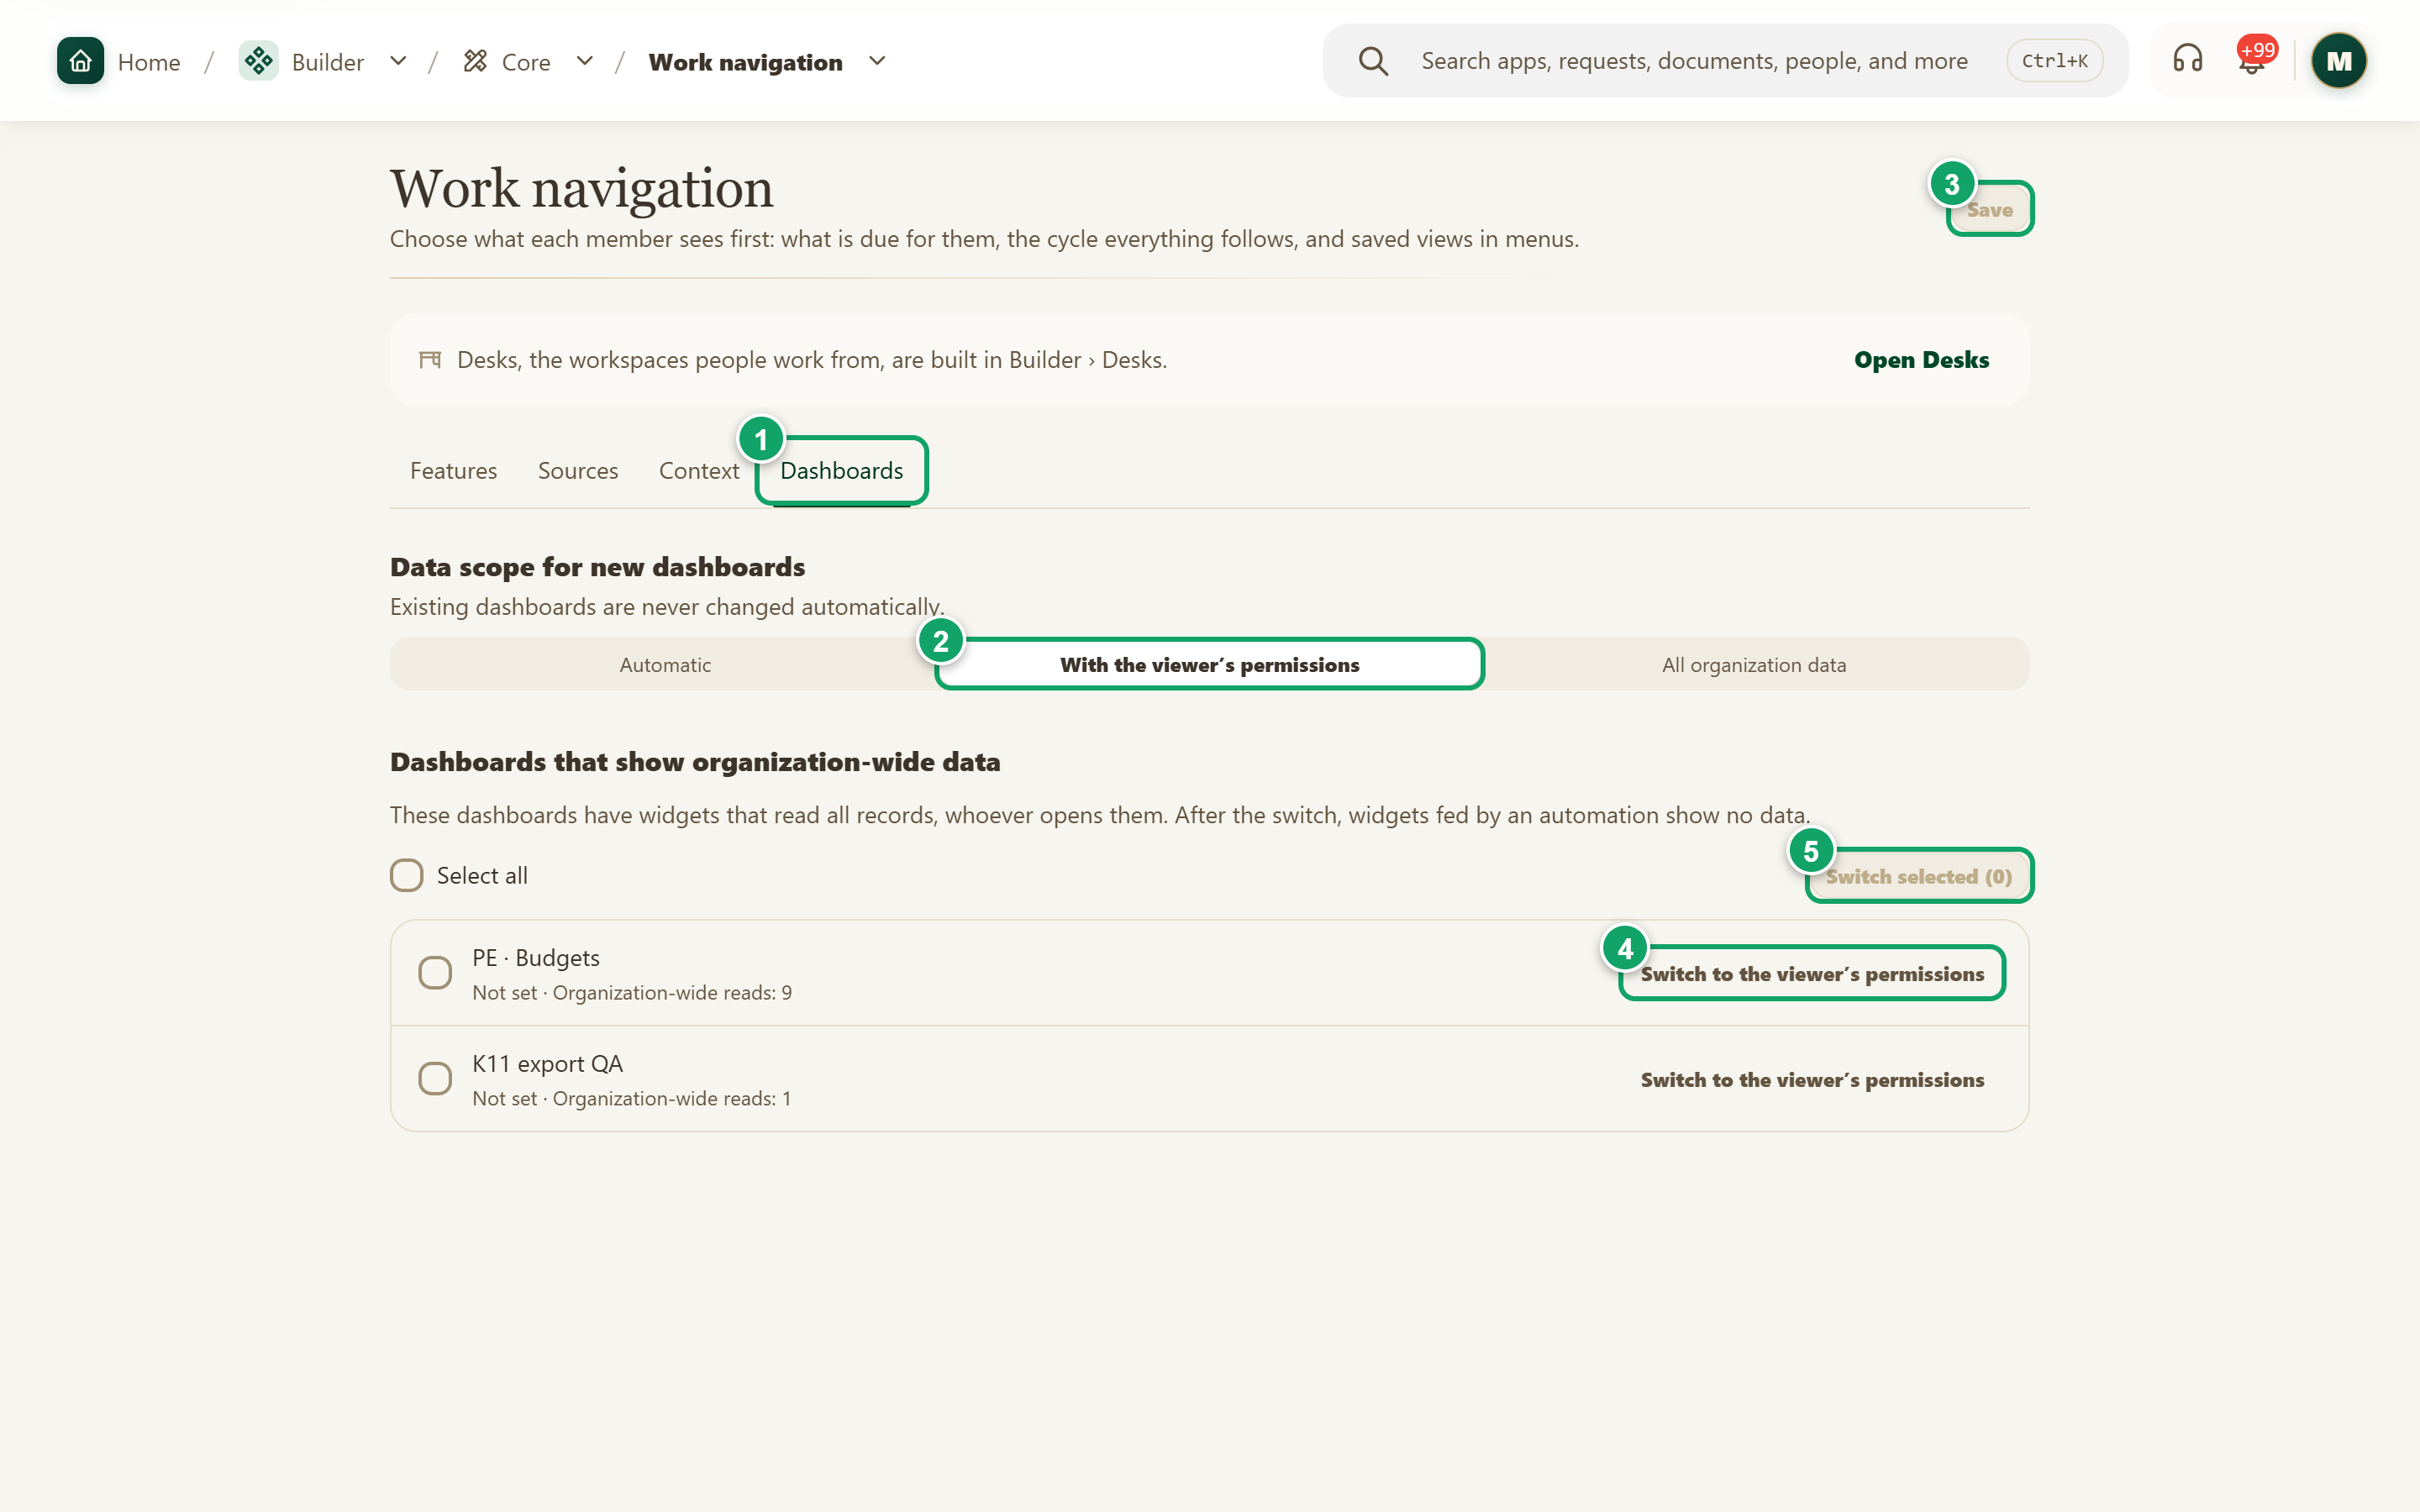
\includegraphics[width=0.95\linewidth,height=0.72\textheight,keepaspectratio]{figures/screens/ch06-wn-dashboards-en.png}
\caption{The “Dashboards” tab}
\label{fig:builder-work-navigation-dashboards-screen}
\shotnote{The image shows the “Dashboards” tab in the test organization, where new dashboards use “With the viewer’s permissions”, while the list still holds two dashboards that read organization-wide data, with the number of such reads. It shows that choosing the scope does not change existing dashboards, and that switching them is a separate step applied at once. ① “Dashboards”: the tab. ② “With the viewer’s permissions”: the scope for new dashboards. ③ “Save”: saves the scope choice. ④ “Switch to the viewer’s permissions”: switches one dashboard. ⑤ “Switch selected”: switches every dashboard you selected.}
\end{figure}

\begin{table}[H]
\centering
\caption{What the “Dashboards” tab holds}
\label{tab:builder-work-navigation-dashboards-parts}
\begin{tabularx}{\linewidth}{R{3.6cm} Y}
\rcHeaderRow
\thh{Part} & \thh{What it does}\\
Data scope for new dashboards & “Automatic”, “With the viewer’s permissions” or “All organization data”. Automatic means the viewer's permissions while any work navigation feature is on. Existing dashboards do not change with this choice.\\
Dashboards that show organization-wide data & A list of dashboards with widgets that read all records whoever opens them, with the number of such reads for each dashboard.\\
Switch to the viewer’s permissions & Switches one dashboard, or “Switch selected” switches every dashboard you selected. The switch applies at once, without waiting for “Save”.\\
\end{tabularx}
\end{table}

\begin{rcwarn}[Before switching]
After the switch, widgets fed by an automation show no data, because automations do not run with the viewer's permissions. So review the dashboard after switching it, and rebuild those widgets if you need them.
\end{rcwarn}

\begin{figure}[H]
\centering
\begin{tikzpicture}[node distance=0.5cm]
\node[stepBox] (a) {Choose the scope for new dashboards};
\node[stepBox,below=of a] (b) {Save};
\node[stepBox,below=of b] (c) {Review the list of dashboards};
\node[stepBox,below=of c] (d) {Switch to the viewer's permissions};
\node[stepBox,below=of d] (e) {Open and review the dashboard};
\draw[flowsTo] (a) -- (b);
\draw[flowsTo] (b) -- (c);
\draw[flowsTo] (c) -- (d);
\draw[flowsTo] (d) -- (e);
\end{tikzpicture}
\rclegend
\caption{Setting the dashboard data scope}
\label{fig:builder-work-navigation-dashboards-flow}
\shotnote{The diagram separates two actions that are saved in different ways: the scope for new dashboards is saved with the rest of the page by “Save”, while the switch applies to the dashboard at once. So the chain ends by opening the dashboard to make sure its widgets still show what is expected of them.}
\end{figure}

\subsection{Steps and check}
\begin{enumerate}
\item Open “Work navigation”, then the “Dashboards” tab.
\item Choose the right value under “Data scope for new dashboards”, then press “Save” in the page header.
\item Review “Dashboards that show organization-wide data”, and select the dashboards that should show each person only what concerns them.
\item Press “Switch to the viewer’s permissions” on the dashboard's row, or “Switch selected”.
\end{enumerate}

\textbf{Check and recovery:} after the switch, the message “Switched to the viewer’s permissions:” appears with the count, and the dashboard leaves the list. When the list is empty, “No dashboard shows organization-wide data.” appears. If “Could not switch the dashboards.” appears, try again; if the list does not show at all, ask the organization owner or an administrator to open the tab.

\clearpage
\section{Settings that need attention}
\label{sec:builder-feature-work-navigation-stale}

“Work navigation” settings point at things that live elsewhere: record types, fields, transitions, roles, apps and sections. If one of them is deleted or its kind changes, the setting that points at it is no longer valid. So the page checks its settings when it opens, and shows what needs fixing before members notice something wrong in their lists.

Saving refuses any setting that points at something missing, so nothing is saved until you fix it.

\textbf{Path and who uses it:} “Builder” → “Core” → “Work navigation”, then the tab marked with the alert. Used by the organization owner and administrator after changing record types or roles.

\begin{rcnote}[Example: Horizon]
The system administrator deletes the “Reviewer” field from “Visit requests”, and “Work navigation” shows “Settings that need attention: 1”. They open “Sources” and find on the source “Field not found” with the reason “the field no longer exists”, so they choose another field and save.
\end{rcnote}

\begin{table}[H]
\centering
\caption{Messages you may see}
\label{tab:builder-work-navigation-stale-messages}
\begin{tabularx}{\linewidth}{R{3.6cm} Y}
\rcHeaderRow
\thh{Message} & \thh{What it means and what to do}\\
Settings that need attention & The number of settings that point at something deleted or changed. Each tab with a problem is marked, and a line under the setting names the item and the reason.\\
The stored settings could not be read & The saved settings are damaged, so every feature behaves as if it were off. Saving here replaces them with what you set on the page.\\
Someone else saved these settings after you opened them & Nothing was saved. Press “Reload” to see their changes; your unsaved edits will be lost.\\
\end{tabularx}
\end{table}

\begin{table}[H]
\centering
\caption{Common reasons}
\label{tab:builder-work-navigation-stale-reasons}
\begin{tabularx}{\linewidth}{R{3.6cm} Y}
\rcHeaderRow
\thh{Reason} & \thh{The fix}\\
The record type no longer exists & Choose another record type for the source or context, or delete the setting.\\
The field no longer exists & Choose the field that replaced it in the source dialog.\\
No longer a status, date, relation or member field & The field's kind changed in the Builder, so choose a field of the required kind.\\
The role, app or section was deleted & Remove the deleted item from “Roles that see it” or from the context's places.\\
\end{tabularx}
\end{table}

\begin{figure}[H]
\centering
\begin{tikzpicture}[node distance=0.5cm]
\node[stepBox] (a) {Read the number of settings};
\node[stepBox,below=of a] (b) {Open the marked tab};
\node[stepBox,below=of b] (c) {Read the item and reason};
\node[stepBox,below=of c] (d) {Edit or delete the setting};
\node[stepBox,below=of d] (e) {Save};
\draw[flowsTo] (a) -- (b);
\draw[flowsTo] (b) -- (c);
\draw[flowsTo] (c) -- (d);
\draw[flowsTo] (d) -- (e);
\end{tikzpicture}
\rclegend
\caption{Fixing a setting that points at a deleted item}
\label{fig:builder-work-navigation-stale-flow}
\shotnote{The diagram shows that the fix starts from the marked tab, because each problem shows next to the setting that caused it. It ends with saving, because the page accepts no other save while a single problem remains.}
\end{figure}

\subsection{Steps and check}
\begin{enumerate}
\item Open “Work navigation” and read the count of “Settings that need attention”.
\item Open the tab carrying the alert mark, and find the red line under the setting.
\item Read the item and the reason, then press “Edit” on the source's row or edit the context directly.
\item Choose an existing item instead of the deleted one, or delete the setting if it is no longer needed, then press “Save”.
\end{enumerate}

\textbf{Check and recovery:} after saving, the “Settings that need attention” message and the tab marks disappear, and “Work navigation saved” appears. If “The settings could not be saved.” appears with “Some settings are not valid:”, read the list that follows and fix each item in it. If the conflict message appears, press “Reload” and then make your edit again.
